% Options for packages loaded elsewhere
\PassOptionsToPackage{unicode}{hyperref}
\PassOptionsToPackage{hyphens}{url}
%
\documentclass[
  11pt,
]{article}
\usepackage{amsmath,amssymb}
\usepackage{lmodern}
\usepackage{iftex}
\ifPDFTeX
  \usepackage[T1]{fontenc}
  \usepackage[utf8]{inputenc}
  \usepackage{textcomp} % provide euro and other symbols
\else % if luatex or xetex
  \usepackage{unicode-math}
  \defaultfontfeatures{Scale=MatchLowercase}
  \defaultfontfeatures[\rmfamily]{Ligatures=TeX,Scale=1}
\fi
% Use upquote if available, for straight quotes in verbatim environments
\IfFileExists{upquote.sty}{\usepackage{upquote}}{}
\IfFileExists{microtype.sty}{% use microtype if available
  \usepackage[]{microtype}
  \UseMicrotypeSet[protrusion]{basicmath} % disable protrusion for tt fonts
}{}
\makeatletter
\@ifundefined{KOMAClassName}{% if non-KOMA class
  \IfFileExists{parskip.sty}{%
    \usepackage{parskip}
  }{% else
    \setlength{\parindent}{0pt}
    \setlength{\parskip}{6pt plus 2pt minus 1pt}}
}{% if KOMA class
  \KOMAoptions{parskip=half}}
\makeatother
\usepackage{xcolor}
\usepackage[margin=1in]{geometry}
\usepackage{graphicx}
\makeatletter
\def\maxwidth{\ifdim\Gin@nat@width>\linewidth\linewidth\else\Gin@nat@width\fi}
\def\maxheight{\ifdim\Gin@nat@height>\textheight\textheight\else\Gin@nat@height\fi}
\makeatother
% Scale images if necessary, so that they will not overflow the page
% margins by default, and it is still possible to overwrite the defaults
% using explicit options in \includegraphics[width, height, ...]{}
\setkeys{Gin}{width=\maxwidth,height=\maxheight,keepaspectratio}
% Set default figure placement to htbp
\makeatletter
\def\fps@figure{htbp}
\makeatother
\setlength{\emergencystretch}{3em} % prevent overfull lines
\providecommand{\tightlist}{%
  \setlength{\itemsep}{0pt}\setlength{\parskip}{0pt}}
\setcounter{secnumdepth}{5}
\newlength{\cslhangindent}
\setlength{\cslhangindent}{1.5em}
\newlength{\csllabelwidth}
\setlength{\csllabelwidth}{3em}
\newlength{\cslentryspacingunit} % times entry-spacing
\setlength{\cslentryspacingunit}{\parskip}
\newenvironment{CSLReferences}[2] % #1 hanging-ident, #2 entry spacing
 {% don't indent paragraphs
  \setlength{\parindent}{0pt}
  % turn on hanging indent if param 1 is 1
  \ifodd #1
  \let\oldpar\par
  \def\par{\hangindent=\cslhangindent\oldpar}
  \fi
  % set entry spacing
  \setlength{\parskip}{#2\cslentryspacingunit}
 }%
 {}
\usepackage{calc}
\newcommand{\CSLBlock}[1]{#1\hfill\break}
\newcommand{\CSLLeftMargin}[1]{\parbox[t]{\csllabelwidth}{#1}}
\newcommand{\CSLRightInline}[1]{\parbox[t]{\linewidth - \csllabelwidth}{#1}\break}
\newcommand{\CSLIndent}[1]{\hspace{\cslhangindent}#1}
\usepackage{float} \usepackage{setspace} \usepackage[nottoc]{tocbibind}
\usepackage{booktabs}
\usepackage{longtable}
\usepackage{array}
\usepackage{multirow}
\usepackage{wrapfig}
\usepackage{float}
\usepackage{colortbl}
\usepackage{pdflscape}
\usepackage{tabu}
\usepackage{threeparttable}
\usepackage{threeparttablex}
\usepackage[normalem]{ulem}
\usepackage{makecell}
\usepackage{xcolor}
\ifLuaTeX
  \usepackage{selnolig}  % disable illegal ligatures
\fi
\IfFileExists{bookmark.sty}{\usepackage{bookmark}}{\usepackage{hyperref}}
\IfFileExists{xurl.sty}{\usepackage{xurl}}{} % add URL line breaks if available
\urlstyle{same} % disable monospaced font for URLs
\hypersetup{
  hidelinks,
  pdfcreator={LaTeX via pandoc}}

\author{}
\date{\vspace{-2.5em}}

\begin{document}

\onehalfspacing

\begin{center}
    {\Large \textbf{Abstract}}
\end{center}

\vspace{0.5cm}

\noindent 

\hfill\break
Freq. Lasso\\
Freq. Elastic Net\\
ML XGboost\\
Bayes. Spike and Slab Prior\\
Bayes. Horsehoe Prior (two packages)\\
Bayes. Horseshoe Prior +\\
Bayes. Spike and Slab Lasso\\
Bayes. Bayesian Lasso\\
Bayes. Laplace Approximation\\
Bayes. Shotgun Stochastic Search\\
\strut \\
\textbf{Include result summary!}\\
This study explores the challenges inherent in variable selection for
linear models in Bayesian statistics, particularly in
high-dimensionality settings using R packages. The term
``high-dimensionality'' here refers to contexts involving many
predictors that are fewer, equal to, or greater than the number of data
points. Frequentist penalised regression methods LASSO and Elastic Net,
and XGBoost Machine Learning methods are initially used to establish a
benchmark. Subsequently, the Bayesian methods used include the Bayesian
Lasso, Spike and Slab prior, Horseshoe priors, Laplace Approximation,
and the recently revised Shotgun Stochastic Search with Screening. The
packages that involve the same methodology are compared to establish
user-friendliness. The thesis compares the methodology using simulated
scenarios and the socioeconomic crime dataset.\\

\newpage

\tableofcontents

\newpage

\section{Acknowledgements}

I am profoundly grateful to my advisor, Dr.~Michail Papathomas, whose
guidance was instrumental throughout my dissertation journey. His
insights and constructive feedback on my draft greatly contributed to my
work. My sincere appreciation goes to the Computer Science laboratory
for providing a conducive environment that promoted privacy and cheerful
atmosphere, free from the constraints of societal norms. A special
mention goes to the new friends I have made over the last year - their
support has been invaluable, and they will forever hold a special place
in my heart. Finally, I would like to express my gratitude to the
beaches of St Andrews, whose breathtaking beauty served as a constant
source of inspiration and tranquility during this period.

\newpage

\section{Introduction}
  \subsection{Personal Interest}

The motivation to delve into the intricacies of the Bayesian statistical
framework was kindled by Nobel laureate Daniel Kahneman's seminal and
highly digestible book `Thinking Fast and Slow'
(\protect\hyperlink{ref-Kahneman2011}{Kahneman, 2011}). Kahneman's
dissection of human cognitive biases and flawed decision-making,
especially in ambiguous situations, characterises System 1 thinking as
heuristic-driven, low-cost, and low-effort, often resulting in pitfalls
of emotionally induced biases. It is posited that the Bayesian
methodology parallels System 2 thinking, where initial prior beliefs are
systematically updated with new evidence, considering the strength of
the information. The Bayesian approach provides an explicit mathematical
framework for handling uncertainty, counterbalancing overconfidence and
confirmation bias by quantifying uncertainties in light of new evidence.

\subsection{Concept Comparison: Bayesian Against Frequentist Against Machine Learning}

Bayesian statistics employs probability distributions, constructed using
probability theory, to describe the `degree of belief'. Its strengths
and weaknesses simultaneously lie in the flexible incorporation of
background information. Arguably, it presents a more organic approach to
scientific reasoning than frequentist methods by continually updating
probability distributions with new data. Focusing solely on the
likelihood of data under specific hypotheses, without incorporating
prior beliefs, leads to a rigid inference process that lacks the
capability for iterative updating of beliefs. Prior beliefs are
particularly advantageous when data is scarce or hard to acquire; using
prior information might be the only option. Even with a non-informative
prior, Bayesian methodology yields a distribution in contrast to the
classical approach's point estimate, making it more intuitively
understandable.

Bayesian approaches elegantly circumvent challenges encountered by
classical methods. They sidestep issues of functional maximisation,
which eliminates problems with algorithm convergence and the delicate
task of choosing starting values close to the maximum
(\protect\hyperlink{ref-Train2012}{Train, 2012}). Further, Bayesian
methods alleviate the dilemma between local and global maxima, as
convergence does not inherently imply the attainment of a global
maximum. Moreover, they allow for desirable consistency and efficiency
under more forgiving conditions: consistency is achievable with a fixed
number of simulation draws, and any increase in draw numbers with sample
size ensures efficiency.

\hypertarget{machine-learning}{%
\subsection{MACHINE LEARNING}\label{machine-learning}}

\subsection{Motivation}

In the realm of data-driven decision-making, substantial emphasis is
placed on the abundance of data. This idea follows the mathematical
principle that the number of observations should generally exceed the
number of explanatory variables, which aids in preventing overfitting in
models and enhances predictive power. Technological advancements have
quickly fueled scientific progress, enabling us to amass large volumes
of data, often with the number of variables greatly exceeding the number
of data points. One of the critical challenges in this high-dimensional
setting is to impose sparsity, a strategy that promotes model simplicity
and interpretability without sacrificing significant predictive
accuracy, thereby addressing the variance and overfitting issues
inherent in high-dimensional data
(\protect\hyperlink{ref-Hastie2017}{Hastie et al., 2017}). For instance,
thousands of noisy pixel observations may exist in astronomy and image
processing, but only a tiny subset is typically required to identify the
objects of interest (\protect\hyperlink{ref-Johnstone2004}{Johnstone \&
Silverman, 2004}). Meanwhile, in medical research involving rare
diseases or novel treatments, data is often scarce, i.e.~there are few
data points. In those instances, the Central Limit Theorem (CLT) of
normality sometimes needs to be more appropriately invoked to make
assumptions about the underlying distribution of the data, despite
insufficient sample sizes for the theorem to hold accurately.

A significant and well-known challenge in high-dimensional model
selection is the issue of collinearity among predictors
(\protect\hyperlink{ref-Jianqing2010}{Jianqing et al., 2010}). This
collinearity can often be misleading, especially in high-dimensional
geometry (\protect\hyperlink{ref-Fan2008}{Fan \& Lv, 2008}), leading to
the selection of an inaccurate model.

This thesis investigates high-dimensionality linear regression variable
selection problems in both simulated data, where the number of
predictors is smaller, equal, greater or even much greater than the
number of data points, and the real data with a large number of
predictors and a larger number of data points. Both will allow the
exploration of issues in high dimensionality. The methods used encompass
a selected handful of Bayesian approaches, classical penalised
regression techniques, and a machine learning ensemble tree, all
implemented using R software. It should be noted that some methodologies
deployed in this study are not the original versions but extensions
found within the implemented packages. This approach is intended to
simplify the reader's narrative and illuminate the adaptations required
to overcome computational limitations, enhance methodological efficiency
and improve performance outcomes. In doing so, this study provides
insights into which adjustments have proved most effective. Furthermore,
comparative analyses of different packages for some methodologies are
undertaken.

The aims of this thesis extend beyond applying and comparing a variety
of Bayesian variable selection methods in linear regression problems.
Equally important is the personal journey into the depth of this
statistical framework. Prior to my Master's degree in Applied Statistics
and Data Mining, my academic foundation was rooted in a creative
discipline. Hence, this exploration of statistical frameworks stands not
only as a scholarly endeavour but also as a pivotal chapter in my
academic transition and growth. Hence, this document delivers a somewhat
more extensive description of the methods, blending theory with
application, to foster a deep understanding of the methodology and its
practical testing.

\subsection{Structure of Thesis}

This thesis is structured as follows: Chapter 1 introduced a succinct
overview of dissertation coupled with a reflection on personal
interests. Chapter 2 delves into a more detailed and formally-structured
motivation for variable selection in high-dimensional setting. Chapter 3
lays the foundation of Bayesian inference theory. Chapter 4 specifically
overviews the variable selection methods within the Bayesian framework
providing mathematical scaffolding and application-motivated package
overview in R. Chapters 5 and 6 explore the application of variable and
model selection in simulated and real high-dimensional data, with focus
on methods that utilise shrinkage priors and penalised regression
techniques. Finally, Chapter 7 provides the discussion of the analysis
and findings.

\newpage

\section{Building Blocks}

This thesis focuses on parametric models, characterised by a finite
number of parameters independent of the sample size, belonging to the
parameterised family of distributions. In contrast, non-parametric
models allow for an adaptable number of parameters as the sample size
expands. Model complexity is reflected by the number of parameters.

To begin with, the steps involved in Bayesian inference methodology are
outlined to facilitate familiarity with the concepts:

\begin{enumerate}
\def\labelenumi{\arabic{enumi}.}
\item
  \emph{Development of a full Probability Model}: A joint probability
  distribution that encompasses all observable and latent variables is
  formulated. Ensuring the model is consistent with the prevailing
  understanding of the scientific problem and the data collection
  procedure is crucial.
\item
  \emph{Conditioning on Observed Data}: The posterior distribution is
  computed and analysed. The most common approach to posterior
  distribution computation is Markov Chain Monte Carlo (MCMC) and Gibbs
  Sampling. Given the observed data, this distribution represents the
  conditional probability of the latent variables of interest.
\item
  \emph{Assessment of Model Fit and Posterior Distribution
  Implications}: The model is evaluated, as are the plausibility of the
  substantive conclusions derived from the posterior distribution. The
  assessment also includes checking the conclusions' robustness and the
  results' sensitivity to the initial modelling assumptions. If
  necessary, the model is then modified or expanded, and the process is
  iterated.
\end{enumerate}

\subsection{Prior Distribution}

The following three sub-chapters are heavily based on Joseph C. Watkins
``Theory of Statistics'' lecture notes from the University of Arizona.

Firstly, a realisation of random variables on a sample space \(X\) is
observed, represented as

\begin{equation}
X(s) = (X_1(s), ..., X_n(s)),
\end{equation}

where each \(X_i\) shares the same distribution. The allowable
distributions are typically restricted to a class \(P\). If these
distributions can be indexed by a set \(\Omega \subset \mathbb{R}^d\),
then \(P\) is termed a parametric family. The indexing is usually set up
to ensure identifiability, i.e., the mapping from \(\Omega\) to \(P\) is
bijective. For a chosen parameter \(\theta \in \Omega\), the
distribution of the observations and the expectation are denoted by
\(P_\theta\) and \(E_\theta\), respectively.

As mentioned in the Chapters XX above, \emph{prior distribution} can be
informed using additional data, expert knowledge, elicitation
techniques, or sometimes, it may be challenging to define. (mention
uninformative priors) In Bayesian statistics, \((X, \Theta)\) is
considered as a pair of random variables with an associated state space
\(X \times \Omega\). The distribution, \(\mu\) of \(\Theta\) over
\(\Omega\), is called the \emph{prior distribution}. The joint
distribution of \((X, \Theta)\) is determined by the prior distribution
in conjunction with the family \(\{P_\theta : \theta \in \Omega\}\):
\begin{equation}
\Pr\{(X,\Theta) \in B\} = \int \int I_B(x,\theta) \mu_{X|\Theta}(dx|\theta) \mu_{\Theta}(d\theta).
\end{equation} Here, \(\mu_{X|\Theta}(\cdot|\theta)\) represents the
distribution of \(X\) under \(P_{\theta}\).

\subsection{Bayes’ Theorem and Posterior Distribution}

Consider the scenario where \(\mu_{\Theta}\) has density \(f_{\Theta}\)
and \(\mu_{X|\Theta}(\cdot|\theta)\) has density \(f_{X|\Theta}\) with
respect to the Lebesgue measure. The probability is then:
\begin{equation}
\Pr\{(X,\Theta) \in B\} = \int\int I_B(x,\theta)f_{X|\Theta}(x|\theta)f_{\Theta}(\theta) \,dx \,d\theta.
\end{equation} The Lebesgue measure, here, serves as a standard way of
assigning a length, area, or volume to subsets of a Euclidean space and
is fundamental in integration theory.\\
After observing \(X = x\), the conditional density of \(\Theta\) given
\(X = x\) using \emph{Bayes' theorem}, the \emph{posterior distribution}
\(f_{\Theta|X}(\theta|x)\) is given as:

\begin{equation}
f_{\Theta|X}(\theta|x) = \frac{f_{X|\Theta}(x|\theta) \cdot f_{\Theta}(\theta)} {\int_{\Omega} f_{X|\Theta}(x|t) \cdot f_{\Theta}(t) \, dt}.
\end{equation}

The term \(f_{X|\Theta}(x|\theta)\) is the likelihood of observing
\(X = x\) given \(\Theta = \theta\), and \(f_{\Theta}(\theta)\) is the
prior density of \(\Theta\). The denominator represents the marginal
likelihood of \(X = x\), a normalising constant to ensure that the
posterior density integrates to 1.

The likelihood function \(f_{X|\Theta}(x|\theta)\) evaluates how
probable the observed data \(x\) is under various parameter values
\(\theta\). Unlike the \emph{prior distribution}, the likelihood
function depends solely on the data and quantifies the support it
provides for various parameter values. It is important to note that the
likelihood function is not a probability distribution over \(\theta\).
That is, it does not provide probabilities for different parameter
values but rather gives a measure of how well each parameter value
\(\theta\) is supported by the data.

Here, it is also important to mention that Bayesian inference obeys The
Likelihood principle, according to which, different probability models
that produce the same likelihood for the data should result in the same
inference for the parameter \(\theta\). The data only influence the
posterior through the likelihood function \(f(x|\theta)\), while the
prior remains independent of the data. Experimental variations are
irrelevant for inference about \(\theta\).

The posterior distribution synthesises all available information
regarding the parameter of interest. However, deriving analytical
summaries, such as the posterior distribution's mean or variance, often
requires evaluating complex integrals. The evaluation can be incredibly
challenging for high-dimensional posterior distributions. Monte Carlo
integration, a simulation technique, offers an effective solution for
estimating these integrals. Within Monte Carlo integration, Markov Chain
Monte Carlo (MCMC) methodology is a powerful tool for approximating
posterior summary statistics, the application of this methodology is
defined in the following Chapter.

\subsection{MCMC Algorithm}

\emph{Markov Chain Monte Carlo (MCMC)} involves generating samples of
\(\theta\) from approximate distributions and iteratively refining these
samples to converge to the desired posterior distribution,
\(p(\theta|y)\). The essence of \emph{MCMC} is not the Markov property
per se but the progressive improvement of the approximation towards the
target distribution with each iteration. A Markov chain is defined as a
stochastic sequence
\(\{\theta^0, \theta^1, \theta^2, \ldots, \theta^n\}\), where each state
\(\theta^n\) depends only on its immediate predecessor \(\theta^{n-1}\),
with the initial state \(\theta^0\) is set to an arbitrary value. The
Markov chain evolves according to a transition kernel \(P\), dependent
only on \(\theta^n\):

\begin{equation}
\theta^{n+1} \sim P(\theta^n, \theta^{n+1}) \, (\equiv P(\theta^{n+1}|\theta^n)).
\end{equation}

Under the conditions of aperiodicity and irreducibility, the
\emph{Markov chain} attains a stationary distribution, independent of
initial values. After discarding initial states, the remaining states
serve as dependent samples from the target posterior distribution. It is
essential to ensure sufficient iterations for convergence and an
adequate post-convergence sample size for minimal \emph{Monte Carlo}
errors. The complexity of the posterior distribution does not
significantly affect the simplicity of state updates in the chain.

Determining the number of initial states to discard, known as burn-in,
is crucial to ensure that the Markov Chain has converged to the
stationary distribution. Two common approaches to assess burn-in are
through trace plots and the Brooks-Gelman-Rubin (BGR) diagnostic.

The number of iterations after burn-in is essential to estimate the
summary statistics accurately, and it is important to evaluate the
\emph{Monte Carlo} error. A common approach to estimating the
\emph{Monte Carlo} error involves batching. The chain is divided into
\(m\) batches, each of length \(T\), so that \(n = mT\). Let
\(\theta_1,\ldots,\theta_m\) be the sample means for each batch, and
\(\theta\) denote the mean overall \(n\) samples. The batch means
estimate of \(\sigma^2\) is then,

\begin{equation}
\hat{\sigma}^2 = \frac{T}{m - 1} \sum_{i=1}^{m}(\bar{\theta}_i - \bar{\theta})^2.
\end{equation}

An estimate of the \emph{Monte Carlo} error is
\(\sqrt{\frac{\hat{\sigma}^2}{n}}\). The efficiency of the Markov chain
in exploring the parameter space can be evaluated using the
autocorrelation function (ACF). The ACF is the correlation of a
parameter's value in the Markov chain with itself at a lag \(j\),
defined as \(\text{cor}(\theta^t, \theta^{t+j})\). Efficient chains show
a fast decrease in ACF as the lag increases, indicating low dependency
between chain values within a few iterations.

An alternative estimate of the Monte Carlo error uses the effective
sample size \(M\), defined as

\begin{equation}
M = \frac{n}{1 + 2 \sum_{k=1}^{\infty} \rho_k},
\end{equation}

where \(\rho_k\) is the autocorrelation at lag \(k\). Practically, \(M\)
is estimated through an alternative method accounting for
autocorrelations. The Monte Carlo error can be estimated as
\(\sqrt{\frac{\hat{\sigma}^2}{\hat{M}}}\).

Thinning is a process of selecting every \(k\)-th realisation to reduce
the autocorrelation of the \emph{MCMC} sample. It is used primarily to
alleviate storage or memory issues but should be used judiciously as
information is lost in the discarded samples.

The description above lays the foundation of MCMC algorithms, of which
three are particularly prominent: Gibbs sampling, Metropolis-Hastings,
and Importance/Rejection sampling. The first two will be described in
more detail. The subsequent Chapter XX will introduce an advanced
extension to the MCMC, namely the Reversible Jump MCMC method involving
Gibbs sampling, which is the most relevant to this paper.

\textbf{CONVERGENCE OF MCMC}

\newpage

\section{The Setting}
  \subsection{Linear Regression in High-Dimensional Setting}

The multivariate linear regression model is described as follows:

\begin{equation}
\mathbf{Y} = \mathbf{X}\boldsymbol{\beta} + \boldsymbol{\epsilon}, \quad \boldsymbol{\epsilon} \sim \mathcal{N}(\mathbf{0}, \sigma^2\mathbf{I}_n)
\end{equation}

In this setup, \(\mathbf{Y} \in \mathbb{R}^n\) is a response vector,
\(\mathbf{X} = [\mathbf{X}_1, ..., \mathbf{X}_p] \in \mathbb{R}^{n \times p}\)
is the given design matrix comprising of \(p\) potential predictors. The
vector
\(\boldsymbol{\beta} = (\beta_1, ..., \beta_p)^T \in \mathbb{R}^p\)
represents the set of regression coefficients that will be estimated.
Lastly, \(\boldsymbol{\epsilon} \in \mathbb{R}^n\) is the noise vector,
constituted by independently distributed normal random variables, each
sharing a common but unknown variance \(\sigma^2\). This thesis
investigates instances where the number of predictors is less than,
equal to, exceeds, or greatly exceed the number of data points.

\subsection{Variable Selection Problem}

Variable selection seeks the optimal subset of predictors and
coefficients to drive the most fitting model for the data. However, it
is essential to remember that the ``best'' model does not claim to
uncover the absolute truth about the underlying natural processes, which
are far too intricate to be fully captured in mathematical terms
(\protect\hyperlink{ref-Ewout2019}{Steyerberg, 2019}). With unseen or
undiscovered predictors, and potential effects too minuscule to
empirically detect, statistical models remain valuable approximations,
drawing from the limited palette of known predictors to paint a feasible
picture of the complex reality. In situations where the vector of
regression coefficients \(\beta\) is large and sparse, i.e., most
elements are zero or negligible, the task of identifying the significant
elements of \(\beta\) becomes particularly important
(\protect\hyperlink{ref-Moran2019}{Moran et al., 2019}). In
high-dimensional scenarios where observations are limited, the crucial
task is variable selection. The goal is to identify a sparse subset of
predictors that adequately capture the true signals within the data,
allowing for the construction of parsimonious, interpretable models that
effectively mitigate overfitting (\protect\hyperlink{ref-Fan2008}{Fan \&
Lv, 2008}).

In Bayesian analysis, a Gaussian likelihood for \(\mathbf{y}\) is
commonly employed, predicated on the normal distribution of errors:

\begin{equation}
\mathbf{y} | (\mathbf{X}, \boldsymbol{\beta}) \sim \mathcal{N}(\mathbf{X}\boldsymbol{\beta}, \sigma^2\mathbf{I}).
\end{equation}

For variable selection, binary indicators \(\gamma_j\) are defined to
identify the non-zero elements of \(\boldsymbol{\beta}\).

\textbf{WRITE EXPRESSION FOR BAYESIAN MODEL EXPLICITLY?} \textbf{WRITE
ABOUT NOISE IN DATA}

\newpage

\section{Model Selection Methodology}

This thesis discusses methods to compute the relative quality of
statistical models, including Akaike information criterion (AIC),
deviance information criterion (DIC), Watanabe--Akaike information
criterion (WAIC), and Bayesian Information Criterion (BIC). While this
thesis focuses on variable selection, the task of model selection is
closely related, and some of the applied R packages use these criteria
(f.e. \emph{`spikeslab'} calculates AIC criteria, see Chapter \(XX\)),
warranting their brief explanation for methodological completeness and
personal understanding.

\subsection{AIC}

The following three sections rely on \emph{`Bayesian Data Analysis'} by
Gelman et al. (\protect\hyperlink{ref-Gelman2020}{Gelman et al., 2020}).

The concept of AIC must first be introduced in order to establish a
foundation for understanding several subsequent criteria in Bayesian
Inference, and to enable comparisons among them. AIC favours models with
good predictive capabilities, penalising those with more parameters,
thereby discouraging overfitting.

In statistical literature, inference for \(\theta\) is typically
summarised using a point estimate, \(\hat{\theta}\), rather than the
full posterior distribution. Often, the maximum likelihood estimate
(MLE) is used as this point estimate. A common approach for calculating
out-of-sample predictive accuracy involves using the log posterior
density of the observed data \(y\) given the point estimate,
\(\log p(y|\hat{\theta})\), and correcting for overfitting bias. When
\(k\) represents the number of estimated parameters, the bias correction
is performed by subtracting \(k\) from the log predictive density based
on the MLE, according to the formula:

\begin{equation}
\widehat{elpd}_{\text{AIC}} = \log p(y|\hat{\theta}_{\text{mle}}) - k.
\end{equation}

\emph{AIC} is then defined as twice the negative of this quantity:

\begin{equation}
\text{AIC} = -2 \log p(y|\hat{\theta}_{\text{mle}}) + 2k.
\end{equation}

Though \emph{AIC's} bias correction is applicable in normal linear
models with known variance and uniform priors, it is not adequate in
Bayesian models. In such cases, the penalty of \(k\) simply does not
accurately represent the effective number of parameters. Hence, other
criteria was introduced.

\subsection{DIC}

\emph{Deviance Information Criterion (DIC)} is, to some degree, a
Bayesian version of \emph{AIC}, two changes are applied: the maximum
likelihood estimate \(\hat{\theta}\) is replaced with the posterior mean
\(\hat{\theta}_{\text{Bayes}} = E(\theta | y)\), while \(k\) is replaced
with a data-based bias correction. The measure of predictive accuracy is
then:

\begin{equation}
\widehat{elpd}_{\text{DIC}} = \log p(y|\hat{\theta}_{\text{Bayes}}) - p_{\text{DIC}},
\end{equation} where \(p_{\text{DIC}}\) is the effective number of
parameters, calculated as,

\begin{equation}
p_{\text{DIC}} = 2\left(\log p(y|\hat{\theta}_{\text{Bayes}}) - E_{\text{post}}\left(\log p(y|\theta)\right)\right),
\end{equation}

where the expectation in the second term is an average of \(\theta\)
over its posterior distribution. The above expression can therefore be
evaluated using simulation, specifically by generating a sequence of
\(S\) samples \(\theta^s\) for \(s = 1, . . . , S\), as

\begin{equation}
p_{\text{DIC, computed}} = 2 \left(\log p(y|\hat{\theta}_{\text{Bayes}}) - \frac{1}{S} \sum_{s=1}^{S} \log p(y|{\theta}^s)\right).
\end{equation}

The measure \emph{DIC} is then defined in terms of the deviance rather
than the log predictive density, as,

\begin{equation}
DIC = -2 \log p(y|\hat{\theta}_{\text{Bayes}}) + 2p_{\text{DIC}}.
\end{equation}

\emph{DIC} is only valid when the posterior distribution is
approximately multivariate normal. In some cases, a negative effective
number of parameters can be obtained. \emph{DIC}, besides being heavily
criticised (please refer to detailed criticisms in Spiegelhalter et
al.(\protect\hyperlink{ref-Spiegelhalter2014}{2014})), it also cannot be
used with discrete parameters since \(E_{\pi}(\theta|x)\) typically does
not coincide with one of the discrete values under consideration.

When considering a vast array of possible models, conducting a fit for
each one against the data may not be feasible due to computational
constraints. Furthermore, the \emph{DIC} does not yield a readily
interpretable quantitative comparison, limiting its practicality in such
situations. An alternative approach for Bayesian model discrimination
that offers more intuitive results is using Bayes Factors (please refer
to description xx sections above) or posterior model probabilities.
These methodologies not only offer quantitative comparisons of
contending models but also facilitate the incorporation of model
averaging concepts, potentially enhancing the overall predictive
strength and robustness of the modelling process.

\subsection{WAIC}

The popularity of \emph{DIC} is primarily due to its ease of calculation
and its inclusion in standard software, while \emph{WAIC}, which
requires Monte Carlo estimation of predictive densities, can be
significantly more challenging to implement robustly
(\protect\hyperlink{ref-Spiegelhalter2014}{Spiegelhalter et al., 2014}).

However, due to the extensive issues with \emph{DIC}, \emph{WAIC} was
introduced as a counterpart. \emph{WAIC} represents a more fully
Bayesian approach designed to estimate the out-of-sample expectation.
This approach begins with the computation of the log pointwise posterior
predictive density, followed by adding a corrective measure for the
effective number of parameters, mitigating potential overfitting.

Among two potential modifications considered, this thesis includes the
more robust alternative, which involves calculating the variance of
individual terms in the log predictive density, summed across all the
\(n\) data points, given as,

\begin{equation}
p_{WAIC2} = \sum_{i=1}^{n} \text{var}_{\text{post}}(\log p(y_i|\theta)).
\end{equation}

Formula XX is then computed by evaluating the posterior variance of the
log predictive density for each data point \(y_i\), that is
\(V_{s=1}^{S}\log p(y_i|\theta^s)\), where \(V_{s=1}^S\) represents the
sample variance given by

\begin{equation}
V_{s=1}^{S}a_s = \frac{1}{S-1}\sum_{s=1}^{S} (a_s - \bar{a})^2.
\end{equation}

The total sum across all data points \(y_i\) gives the effective number
of parameters, as,

\begin{equation}
\text{computed } p_{WAIC2} = \sum_{i=1}^{n} V_{s=1}^{S} (\log p(y_i |\theta^s)).
\end{equation}

Then use it for bias correction, as,

\begin{equation}
\widehat{\text{elppd}}_{\text{WAIC}} = \text{lppd} - \text{p}_{\text{WAIC}}.
\end{equation}

Similar to \emph{AIC} and \emph{DIC}, the \emph{WAIC} is determined by
multiplying the above-mentioned expression by negative two to align it
with the deviance scale:

\begin{equation}
WAIC = -2\text{lppd} + 2\text{p}_{WAIC2},
\end{equation}

with \(lppd\) computed as in XX and \(p_{WAIC2}\) in XX.

In contrast to \emph{AIC} and \emph{DIC}, \emph{WAIC} favourably
averages over the posterior distribution instead of relying on a single
point estimate. This characteristic is particularly significant in a
predictive framework as \emph{WAIC} assesses the actual predictions
being made for new data in a Bayesian context. While \emph{AIC} and
\emph{DIC} gauge the performance of the plug-in predictive density,
Bayesian applications of these metrics still employ the posterior
predictive density for forecasting.

\emph{AIC}, \emph{DIC}, and \emph{WAIC} all aim to estimate the same
thing: the expected out-of-sample deviance of a model, which can be
considered as different versions of cross-validation. On the other hand,
\emph{BIC} diverges by being motivated not by predictive fit estimation
but by the objective of approximating the marginal probability density
of the data under the model, pertinent in the context of discrete model
comparison.

\subsection{Bayes’ Factor}

The \emph{Bayes factor}, introduced by Jeffrey
(\protect\hyperlink{ref-jeffreys1935}{1935}), is a key tool in
traditional Bayesian model comparison, widely discussed in Bayesian
literature. It quantifies the relative evidence for two models, \(M_i\)
and \(M_j\), given data \(y\),

\begin{equation}
B_{ij} = \frac{p(y|M_i)}{p(y|M_j)} = \frac{\int p(y|\theta_i,M_i)p(\theta_i|M_i)d\theta_i}{\int p(y|\theta_j,M_j)p(\theta_j|M_j)d\theta_j},
\end{equation}

where \(p(y|\theta_k,M_k)\) denotes the likelihood under model \(k\),
and \(p(\theta_k|M_k)\) represents the prior distribution of
\(\theta_k\). The variable \(M\) denotes the model, taking values from a
finite set of \(K\) models. \emph{Bayes factors} can be derived from
posterior model probabilities with known prior model probabilities
(\protect\hyperlink{ref-Kass1995}{Kass \& Raftery, 1995}), enabling
Bayesian model averaging, which accounts for model uncertainty in
posterior estimates (\protect\hyperlink{ref-Hoeting1999}{Hoeting et al.,
1999}).

Evaluating \emph{Bayes factors} is challenging due to the difficulty in
computing marginal likelihoods for each model. \emph{MCMC} methods offer
a solution but necessitate careful handling of varying parameter numbers
to ensure ergodicity in the Markov chain. Carlin and Chib
(\protect\hyperlink{ref-Carlin1995}{1995}) presented a method involving
a global model with `pseudo-priors' for all parameters. Green's
(\protect\hyperlink{ref-Green1995}{1995}) \emph{Reversible Jump MCMC
(RJMCMC)} employs auxiliary variables to manage model dimension changes.
However, defining pseudo-priors or auxiliary variables can be
challenging and is an area of ongoing research. Barker \& Link
(\protect\hyperlink{ref-Barker2013}{2013}) introduced a simplified
\emph{RJMCMC} approach compatible with Gibbs sampling. Chapter XX
discusses Barker \& Link's approach, its integration with prior
\emph{MCMC} results, and introduces the \emph{RJMCMC} algorithm along
with the \texttt{rjmcmc} R package that facilitates \emph{Bayes factor}
and posterior model probability calculations using \emph{RJMCMC}
outputs.

\subsection{RJMCMC}

The Reversible Jump Markov Chain Monte Carlo (RJMCMC) method, suggested
as a potential methodology within the scope of this dissertation, was
explored. The RJMCMC refines the Metropolis-Hastings algorithm by
facilitating the constructed Markov chain traversing varying dimensions.

As this methodology is still very much under development, the outline is
based on the work of Gelling, Schofield and Barker for the R package
\emph{`rjmcmc'} (\protect\hyperlink{ref-Gelling2019}{Gelling et al.,
2019}). Barker and Link (\protect\hyperlink{ref-Barker2013}{2013})
introduced a modified version of
Green's(\protect\hyperlink{ref-Green1995}{1995}) RJMCMC algorithm which
is compatible with Gibbs sampling, specifically suited for
high-dimensional models.

Given data \(y\) with models indexed \(1,...,K\), and a set of
model-specific parameters \(\theta_k\) for each model \(k\), along with
prior model probabilities \(p(M_k)\), the posterior model probabilities
are related to Bayes factors as:

\begin{equation}
\frac{p(M_i|y)}{p(M_j|y)} = B_{ij} \times \frac{p(M_i)}{p(M_j)}
\end{equation}

\emph{RJMCMC}, as proposed by Green
(\protect\hyperlink{ref-Green1995}{1995}), enables sampling across
models by considering the model indicator as a latent variable that is
sampled using MCMC. Transition between models \(i\) and \(j\)
necessitates that: both models have an equal number of parameters, and a
bijective mapping exists between the parameters of the two models.
Auxiliary variables \(u_i\) are introduced to ensure the dimensions
match, i.e., \(\text{dim}(\theta_i,u_i) = \text{dim}(\theta_j,u_j)\).
With the freedom to transition between any pair of models, \(K(K-1)/2\)
bijections must be defined. The choice of auxiliary variables and
bijections does not alter the posterior distribution, but affects
computational efficiency. Limiting transitions between models can reduce
the number of required bijections.\\
\emph{Insert a graph here}\\
During the \(t\) iteration of the Markov chain, a proposed model
\(M_{j}^*\) is introduced, while the current value is denoted as
\(M_{i}^{(t-1)}\). For model \(M_{j}^*\), the proposed parameter values
are determined using the bijection \(f_{ij}(\cdot)\) as

\begin{equation}
(\theta_{j}^*, u_{j}^*) = f_{ij}(\theta_{i}^{(t-1)}, u_{i}^{(t-1)}).
\end{equation}

The joint proposal is accepted or rejected using a Metropolis step. The
selection of the bijection is crucial, as it affects the efficiency and
convergence rate of the chain. Barker and Link
(\protect\hyperlink{ref-Barker2013}{2013}) introduced a restricted
version of Green's \emph{RJMCMC} algorithm, suitable for implementation
via Gibbs sampling. This method involves introducing a universal
parameter vector \(\psi\), whose dimension is at least the maximum
dimension of the model-specific parameters, i.e.,

\begin{equation}
\text{dim}(\psi) \geq \max_{k} \{\text{dim}(\theta_{k})\}.
\end{equation}

Model-specific parameters \(\theta_i\) and auxiliary variables \(u_i\)
are derived from \(\psi\) using a bijection \(g_i(\cdot)\):

\begin{equation}
(\theta_{i}, u_{i}) = g_{i}(\psi),
\end{equation}

\begin{equation}
\psi = g_{i}^{-1}(\theta_{i}, u_{i}).
\end{equation}

Model parameters in model \(i\) are mapped to model \(j\) through the
universal parameter vector \(\psi\),

\begin{equation}
\begin{split}
(\theta_{j}, u_{j}) &= g_{j}(\psi) \\
                    &= g_{j}(g_{i}^{-1}(\theta_{i}, u_{i})).
\end{split}
\end{equation}

This method necessitates \(K\) bijections to move among \(K\) models.
The joint distribution is expressed as:

\begin{equation}
p(y,\psi,M_k)=p(y|\psi,M_k)p(\psi|M_k)p(M_k),
\end{equation}

where \(p(y|\psi,M_k)=p(y|\theta_k,M_k)\) is the joint probability
density for the data under model \(k\), \(p(\psi|M_k)\) is the prior for
\(\psi\) given model \(k\), and \(p(M_k)\) is the prior model
probability for model \(k\).

Since priors are typically in the form \(p(\theta_k|M_k)\),
\(p(\psi|M_k)\) is found as: \begin{equation}
p(\psi|M_k) = p(g_k(\psi)|M_k) \left| \frac{\partial g_k(\psi)}{\partial \psi} \right|,
\end{equation}

where \(\left| \frac{\partial g_k(\psi)}{\partial \psi} \right|\)is the
determinant of the Jacobian for the bijection \(g_k\), later denoted as
\(|J_k|\). The algorithm employs a Gibbs sampler that alternates between
updating \(M\) and \(\psi\). The full-conditional distribution for \(M\)
is categorical, with probabilities:

\begin{equation}
p(M_k|\cdot) = \frac{p(y,\psi,M_k)}{\sum_j p(y,\psi,M_j)}.
\end{equation}

A sample from the full-conditional for \(\psi\) is obtained by drawing
\(\theta_k\) and \(u_k\) from their respective distributions and
computing \(\psi=g_k^{-1}(\theta_k,u_k)\). Barker and Link
(\protect\hyperlink{ref-Barker2013}{2013}) also detailed a
Rao-Blackwellized estimator for posterior model probabilities, based on
estimating a transition matrix whose \((i, j)\) entry represents the
probability of transitioning from model \(M_i\) to \(M_j\). The
posterior model probabilities are derived by normalising the left
eigenvector of this estimated transition matrix.

An essential feature of the \emph{`rjmcmc'} package is the automatic
computation of \(|J_k|\) through automatic differentiation, which
greatly simplifies implementation, especially when dealing with a large
number of parameters.

Bayes factors computation is challenging, often limiting Bayesian
multimodel inference. The \emph{`rjmcmc'} package facilitates precise
estimation of Bayes factors and posterior model probabilities for a
predefined set of models. While RJMCMC is a versatile algorithm,
allowing parameter changes in MCMC simulations, the \emph{`rjmcmc'}
package is tailored to refine posterior distributions and facilitate
model comparison. Notably, it only permits transitions between models
with an equal number of parameters.

It remains a developing technique, which suggests the need for further
refinement. Comprehensive domain knowledge of the socio-economic data
analysed in later chapters was necessary, including the ability to
pre-select variables, a requirement that could only partially be met.
Prioritising established methodologies ensured reliability in the
findings of this dissertation.

\section{Variable Selection Methodology}

To provide a comprehensive perspective in this thesis, a comparison will
be drawn between the classical statistical methods of variable
selection, one machine learning method, and some traditional and more
modern Bayesian techniques. The output of Bayesian analysis can often be
more intuitive to interpret than the output of a frequentist analysis.
Posterior distributions provide a probability distribution for each
parameter, which tells what values are plausible given the data and the
model. In the classical approach to statistical analysis, variable
selection typically hinges on point estimates of parameters, which are
then subjected to hypothesis testing to determine their significance
(\protect\hyperlink{ref-Krantz1999}{Krantz, 1999}). Notably, a
\emph{p-value}, standing alone, does not constitute a robust measure of
evidence in support of a particular model or hypothesis, which may lead
to misinterpretation (often among non-statisticians) around direct
evidence about the null hypothesis
(\protect\hyperlink{ref-Tanha2017}{Tanha et al., 2017}).

\subsection{Penalised Regression Methods}

In penalised regression methods, a penalty term is added to the
log-likelihood function to enforce a trade-off between bias and variance
in regression coefficients, consequently optimising prediction error.

\textbf{Least Absolute Shrinkage and Selection Operator (LASSO)}
incorporates the \emph{L1-norm}, originally proposed by Tibshirani
(\protect\hyperlink{ref-Tibshirani1996}{1996}), of regression
coefficients (excluding the intercept) as the penalty term:

\begin{equation}
- \log L + \lambda \sum_{j=1}^{p} |\beta_j|, \quad \lambda > 0.
\end{equation}

This penalisation shrinks coefficients toward zero and sets those with a
negligible predictive contribution to zero, serving as an embedded
feature selection method. When the number of predictors, \(p\), exceeds
the number of observations, \(n\), \emph{LASSO} selects at most \(n\)
variables. \emph{LASSO} does not group predictors, often arbitrarily
selecting one from a group of highly correlated predictors.

\textbf{Ridge regression} employs the L2-norm of regression coefficients
(excluding the intercept) as the penalty:

\begin{equation}
- \log L + \lambda \sum_{j=1}^{p} \beta_j^2, \quad \lambda > 0.
\end{equation}

\emph{Ridge regression} shrinks coefficients towards zero but retains
all predictors in the model. When \(n > p\) and there is high
multicollinearity, \emph{Ridge regression} often offers superior
predictions. Note that since the penalty term is the sum of squared
coefficients, shrinkage would not be fair across predictors with
different scales. Hence, they need to be standardised.

\textbf{Elastic Net} combines the L1-norm and L2-norm penalties, the
method first proposed by Zuo and Hastie
(\protect\hyperlink{ref-Zuo2005}{\textbf{Zuo2005?}}):

\begin{equation}
- \log L + \lambda_1 \sum_{j=1}^{p} |\beta_j| + \lambda_2 \sum_{j=1}^{p} \beta_j^2, \quad \lambda_1, \lambda_2 > 0.
\end{equation}

The combination of penalties can also be expressed as:

\begin{equation}
\lambda \left( \alpha \sum_{j=1}^{p} |\beta_j| + \frac{1-\alpha}{2} \sum_{j=1}^{p} \beta_j^2 \right), \quad \lambda > 0, \ 0 \leq \alpha \leq 1.
\end{equation}

Here, \(\alpha\) controls the mixing of \emph{LASSO} and \emph{Ridge}
penalties, and \(\lambda\) regulates the overall strength of
regularisation.

The \emph{`glmnet'} package in R provides efficient procedures for
fitting generalised linear and similar models using penalised maximum
likelihood, allowing for lasso or elastic-net regularisation with a
spectrum of lambda values, and includes capabilities for prediction,
plotting, and cross-validation, even for sparse datasets.

\begin{figure}

{\centering 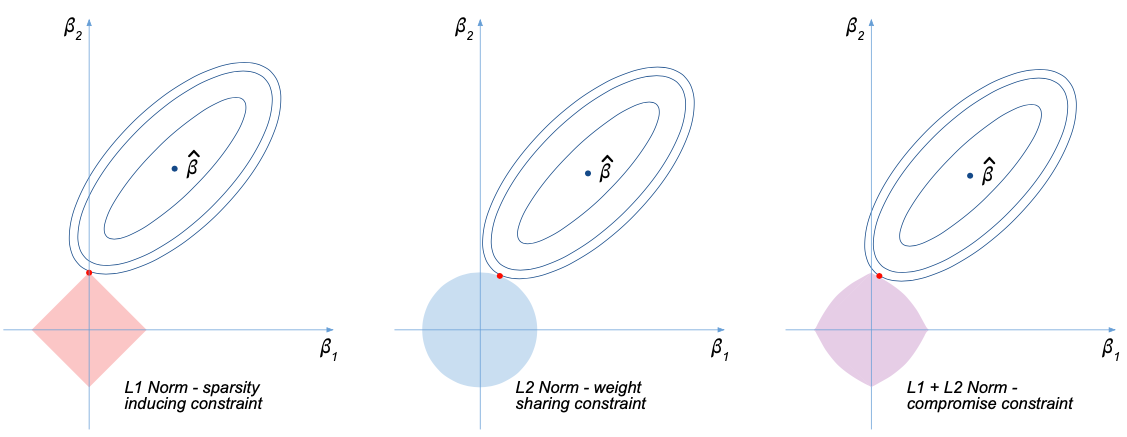
\includegraphics[width=1\linewidth]{reg_pen} 

}

\caption{Penalised Regression}\label{fig:penalisation graphics}
\end{figure}

Despite its proven efficacy, the original Lasso method has certain
constraints. Tibshirani (\protect\hyperlink{ref-Tibshirani1996}{1996})
noted that ridge regression surpasses Lasso when dealing with
multicollinearity among predictors. In situations with more predictors
than observations, namely \(p > n\), Lasso's convex optimisation limits
it to selecting no more than n variables. Moreover, it disregards any
meaningful feature ordering and struggles to effectively select highly
correlated grouped variables, tending to choose individual ones instead.
Later, Meier et al.
(\protect\hyperlink{ref-Merier2008}{\textbf{Merier2008?}}) introduced
algorithms designed for extremely high-dimensional problems to solve
convex optimisation issues. They demonstrated that the group lasso
estimator for logistic regression remains statistically consistent with
a sparse true underlying structure, even when the number of predictors
significantly outnumbers the observations \(p >> n\).

\subsection{Machine Learning}

In exploring variable selection methods, comparing frequentist and
Bayesian inference approaches with a renowned machine learning method,
\emph{XGBoost}, would offer valuable insights. \emph{XGBoost} introduced
by Chen and Guestrin (\protect\hyperlink{ref-Chen2016}{2016}) is often
cited for its outstanding performance in Kaggle competitions/ The method
incorporates a feature importance mechanism, which, in simple terms,
quantifies the contribution of individual attributes to the construction
of decision trees within the ensemble
(\protect\hyperlink{ref-Chen2016}{Chen \& Guestrin, 2016}).

\emph{XGBoost} boasts exceptional scalability, enabling rapid processing
on single machines and adept scaling to billions of examples in
memory-constrained environments. As a comprehensive tree-boosting
system, it introduces innovations such as a sparsity-aware algorithm for
sparse data and a theoretically grounded weighted quantile sketch for
handling instance weights, effectively streamlining resource employment
in processing large datasets (\protect\hyperlink{ref-Chen2016}{Chen \&
Guestrin, 2016}).

The following methodology is based on Wang, Xu, Zhao, Peng and Wang's
definition (\protect\hyperlink{ref-Wang2019}{2019}).

In this thesis, the \emph{XGBoost} model is first classified based on
all features. Secondly, all the importances of feature variables are
computed and then sorted in descending order based on their information
in the generated model process. Lastly, the features are filtered using
a THRESHOLD XX and are inputted into the final model. The \emph{XGBoost}
model has the advantage of high accuracy and is not easy to overfit. It
supports weak classification algorithm and weak regression model and is
suitable for establishing regression model. The model is presented as
follows:

\begin{equation}
\hat{y_i} = \sum_{k=1}^{K} f_k(x_i), \quad f_k \in \mathcal{F}
\end{equation}

where \(\hat{y}_i\) is the predicted value for the \(i\)-th instance,
\(K\) denotes the number of trees, \(\mathcal{F}\) denotes the set of
all possible regression trees, and \(f_k\) represents a specific
regression tree.

The goal of \emph{XGBoost} is to build a \(K\) regression tree such that
the predictions of the tree group are as close as possible to the true
values while ensuring the greatest generalisation ability. The
prediction process is achieved by minimising an objective function,
given by:

\begin{equation}
\text{obj}(\theta) = \sum_{i}^{n} l(y_i, \hat{y}_i) + \sum_{k=1}^{K} \Omega(f_k),
\end{equation}

where the first component, \(\sum_{i=1}^{n} l(y_i, \hat{y}i)\), is a
loss function that measures the deviation of the predicted values from
the true values; the second part, \(\sum_{k=1}^{K} \Omega(f_k)\), acts
as a regularisation term that controls the complexity of the model, as:

\begin{equation}
\Omega(f_k) = \gamma T + \frac{1}{2} \lambda \lVert w \rVert^2,
\end{equation}

where \(T\) represents the number of leave nodes in the tree, and
\(\lVert w \rVert^2\) is the weight of the corresponding leaf nodes.

During the \(t\)-th iteration of training, the objective function is
defined as:

\begin{equation}
\text{obj}^{(t)} = \sum_{i=1}^{n} l\left(y_i, \hat{y}_i^{(t-1)} + f_t(x_i)\right) + \Omega(f_k) + \sum_{i=1}^{t-1} \Omega(f_i)
\end{equation}

This formulation encapsulates each tree's training error and complexity,
steering the algorithm toward building an ensemble of trees that
effectively balances accuracy and generalisation.

Figure XX illustrates the tree-boosting process, based on Guo et al.
(\protect\hyperlink{ref-Guo2020}{2020}).

\begin{figure}[H]

{\centering 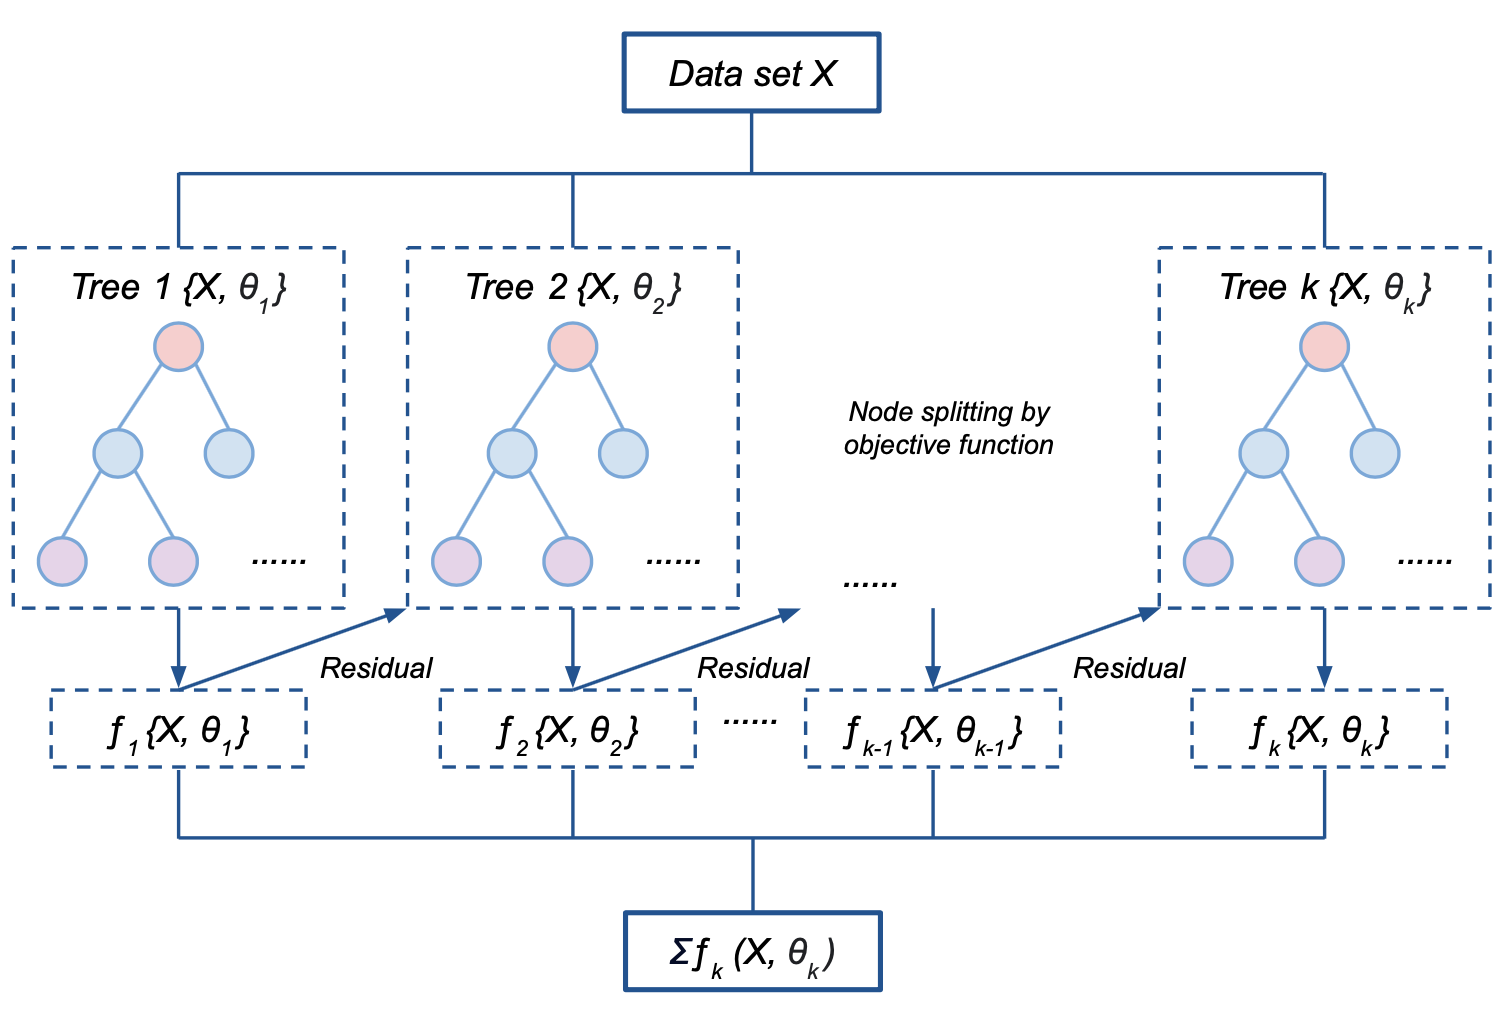
\includegraphics[width=0.9\linewidth]{xgboost_flow} 

}

\caption{XGBoost Algorithm: Iterative Tree Building Process}\label{fig:XGBoost flow}
\end{figure}

While \emph{XGBoost} is acknowledged for its efficacy in classification
tasks, its application for regression with continuous outcomes in
high-dimensionality settings is debated among the data analytics
community as per various informal yet esteemed sources
(\protect\hyperlink{ref-Li2020}{Li, 2020}). A caveat associated with
\emph{XGBoost} is its suboptimal performance when the number of features
surpasses the number of observations in the training data. In this
study, the real dataset being investigated comprises a scenario where
the number of data points exceeds the number of features, albeit with a
high dimensional feature space. It was deemed essential to incorporate
an additional augmented simulated dataset configuration defined in
Chapter XX.

\subsection{Bayesian Framework}

\subsubsection{Bayesian Lasso}

Building on the frequentist penalised regression LASSO, which minimises
the Residual Sum of Squares (RSS) subject to the non-differentiable
constraint expressed in terms of earlier defined L1-norm of the
coefficients, achieve:

\begin{equation}
\min_{\beta} \left(\tilde{y} - X\beta \right)^T \left(\tilde{y} - X\beta \right) + \lambda \sum_{j=1}^{p} |\beta_j|
\end{equation}

where \(\tilde{y} = y - \bar{y}1_n\) for some \(\lambda \geq 0\).

Tibshirani {[}-@ Tibshirani1996{]} interpreted the lasso estimates as
Bayes posterior mode under individual Laplace priors for each predictor.
The Laplace distribution's ability to manifest as a scale mixture of
normal distributions with independently exponentially distributed
variances offers advantages. It prompted several researchers to adopt
Laplace priors within a hierarchical Bayesian framework. This thesis
discusses the one that the \emph{`monomvn'} package implements. Park and
Casella (\protect\hyperlink{ref-Park2008}{\textbf{Park2008?}}) proposed
Gibbs sampling for the LASSO, incorporating a Laplace prior within the
hierarchical model. They considered a fully Bayesian analysis using a
conditional Laplace prior, as:

\begin{equation}
\pi(\beta|\sigma^2) = \prod_{j=1}^{p} \frac{\lambda}{2\sigma} e^{-\lambda|\beta_j|/\sigma}
\end{equation}

where the noninformative, scale-invariant marginal prior is
\(\pi(\sigma^2) = \frac{1}{\sigma^2}\). The conditioning on \(\sigma^2\)
asserts that it secures a unimodal full posterior. A lack of unimodality
can hinder the convergence of the Gibbs sampler, thus rendering point
estimates less reliable. Park and Casella
(\protect\hyperlink{ref-Park2008}{\textbf{Park2008?}}) argue that the
Bayesian Lasso offers a middle ground between Lasso and Ridge regression
by providing smooth paths similar to Ridge but with a tendency to push
less significant parameters towards zero faster, akin to Lasso. This
behaviour suggests an edge of the Laplace prior over Gaussian or
Student-t priors in rapidly diminishing weakly related parameters.

\begin{figure}

{\centering 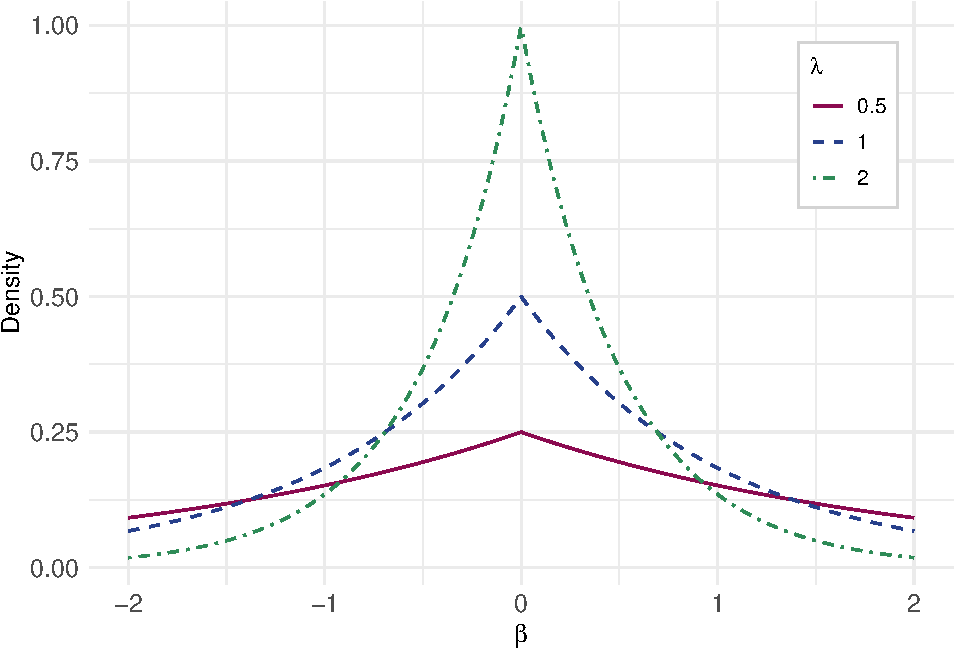
\includegraphics[width=0.85\linewidth]{dissertation_files/figure-latex/Bayesian Lasso Priors-1} 

}

\caption{Density Plots of Laplace Prior Distributions for Bayesian Lasso: Impact of tau}\label{fig:Bayesian Lasso Priors}
\end{figure}

The \emph{'monomvn'} package implements the Bayesian Lasso model using
the Gibbs Sampling algorithm, as described by Park and Casella
(\protect\hyperlink{ref-Park2008}{\textbf{Park2008?}}). It introduced a
feature to use a Rao-Blackwellized sample of \(\sigma^2\), with
\(\beta\) integrated out, to improve the mixing of the sampling
algorithm. A unique feature of this package is the inclusion of
Reversible Jump (RJ) MCMC for Bayesian model selection and averaging,
which allows users to determine the best model based on the columns of
the design matrix and their corresponding \(\beta\) parameters. Unlike
Hans (\protect\hyperlink{ref-Hans2009}{\textbf{Hans2009?}}) and Geweke
(\protect\hyperlink{ref-Geweke1996}{\textbf{Geweke1996?}}) methods,
which require a specific prior on each \(\beta_i\) and individual
conditional sampling, this implementation maintains joint sampling from
the full \(\beta\) vector of non-zero entries, thus facilitating better
Markov chain mixing. It also allows RJ proposals to alter the count of
non-zero entries on a component-wise basis, with high acceptance rates
due to marginalised between-model moves.

\subsubsection{Spike and Slab Prior}

The \emph{spike-and-slab} approach was initially pioneered by Lempers
(\protect\hyperlink{ref-Lempers1971}{1971}), Mitchell, and Beauchamp
(\protect\hyperlink{ref-Mitchell1988}{Mitchell \& Beauchamp, 1988}). The
expression `spike and slab' was characterised by a two-component mixture
prior for \(\beta\). This prior was set such that the \(\beta_k\)
elements were mutually independent, consisting of a flat uniform
distribution (the slab) and a zero degenerate distribution (the spike).
See Figure XX that illustrates two samples drawn from normal
distributions, representing the `spike' and the `slab'. The `spike' is a
sample drawn from a distribution with a small standard deviation,
representing the zero degenerate distribution in the spike-and-slab
prior. The `slab' is a sample drawn from a distribution with a large
standard deviation, representing the flat uniform distribution in the
prior.

\begin{figure}

{\centering 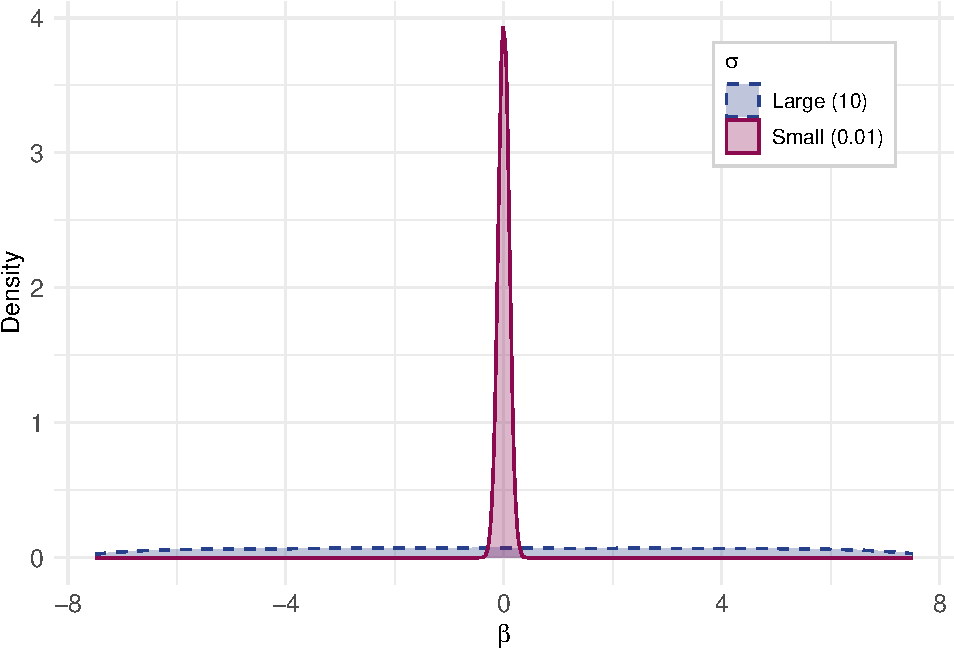
\includegraphics[width=0.75\linewidth]{dissertation_files/figure-latex/Spike Slab Priors-1} 

}

\caption{Density Plots of Three Spike-and-Slab Variants}\label{fig:Spike Slab Priors}
\end{figure}

Ishwaran and Rao (\protect\hyperlink{ref-Ishwaran2005}{2005}) proposed a
departure from this design. Instead of a two-component mixture, they
posited a multivariate normal scale mixture distribution for \(\beta\),
dictated by the prior \(\pi\) for the hypervariance \(\gamma\). Despite
the divergence in distribution choice, the core principle paralleled the
original methodology, aiming to shrink truly zero \(\beta_k\)
coefficients via small posterior mean values. The hypervariances played
a vital role in this, with smaller values driving coefficient shrinkage
and larger ones inflating coefficients for final model selection.

In a further development of the \emph{spike-and-slab} model, Ishwaran
and Rao (\protect\hyperlink{ref-Ishwaran2005}{2005}) introduced a
continuous bimodal prior in a rescaled variant of the model. The use of
such a flexible prior helps to alleviate calibration challenges. To
prevent the diminishing influence of the prior on the posterior as the
sample size increases, they proposed a modification: a sample size
invariant or `universal' rescaling of the spike-and-slab model. This
modification entails transforming the original \(Y_i\) values by a
factor of \(\sqrt{n}\) and incorporating a variance inflation factor to
compensate for the altered variance of the transformed data. The chosen
inflation factor can be viewed as a penalisation shrinkage effect of the
posterior mean. They demonstrated that selecting \(n\) as the inflation
factor ensures that the prior continues to influence the posterior,
avoiding a vanishing effect. Coupled with a suitably chosen prior for
\(\gamma\), this ensures a robust model selection procedure based on the
posterior mean, yielding superior performance over ordinary least
squares (OLS) methods.

The rescaled \emph{spike-and-slab} model is defined by a Bayesian
hierarchical structure as follows
(\protect\hyperlink{ref-Ishwaran2005}{Ishwaran \& Rao, 2005}):

\begin{align*}
    (Y_i^* | x_i, \boldsymbol{\beta}, \sigma^2) &\stackrel{ind}\sim \mathcal{N}(x_i^t \boldsymbol{\beta}, \sigma^2 \lambda_n), \quad i = 1, \ldots, n, \\
    (\boldsymbol{\beta} | \boldsymbol{\gamma}) &\sim \mathcal{N}(\mathbf{0}, \boldsymbol{\Gamma}), \quad \boldsymbol{\Gamma} = \text{diag}(\gamma_1, \ldots, \gamma_K), \\
    \boldsymbol{\gamma} &\sim \pi(d\boldsymbol{\gamma}), \\
    \sigma^2 &\sim \mu(d\sigma^2),
\end{align*}

where the values of \(Y_i^* = \hat{\sigma}_n^{-1} n^{1/2} Y_i\) are
scaled versions of the original response \(Y_i\), where
\(\hat{\sigma}_n^2 = ||Y-X\hat{\beta}_n^{\circ}||^2 / (n-K)\) serves as
an unbiased estimate for \(\sigma_0^2\) based on the full model, and
\(\hat{\beta}_n^{\circ} = (X^tX)^{-1} X^tY\) is the ordinary least
squares estimate for \(\beta_0\). Here, \(\lambda_n\) is a variance
inflation factor introduced to account for the scaling of the \(Y_i\)'s.
While a natural choice for \(\lambda_n\) might be \(n\), to match the
\(\sqrt{n}\)-scaling, \(\lambda_n\) also plays a critical role in
controlling the increase in the variance of the data. In this context,
\(\lambda_n = n\) represents the amount of penalisation necessary to
guarantee a significant shrinkage effect in the limit.

The \emph{'spikeslab'} package, developed by Ishwaran, Kogalur and Rao
(\protect\hyperlink{ref-Ishwaran2010}{2010}), implements a rescaled
three-step spike and slab algorithm using the generalised elastic net
(gnet) and Bayesian model averages (BMA) estimator. The BMA estimator
effectively addresses correlation issues, particularly prevalent in
high-dimensional datasets, leveraging the strengths of weighted
generalised ridge regression (WGRR) - a fundamental advantage of the
Bayesian approach. On the other hand, the gnet estimator applies the
principle of soft-thresholding, a potent frequentist regularisation
concept, to achieve sparse variable selection in complex,
high-dimensional data settings.

The algorithm that underlines the package involved three main steps:
First, variables are filtered down to the top \(nF\), where \(n\) is the
sample size and \(F > 0\) is the user-specified fraction, and ordered
based on absolute posterior mean coefficient value, computed via Gibbs
sampling applied to an approximate rescaled spike and slab posterior.
The user is provided with an option to engage this filtering step when
\(p \geq n\), but it should be noted that in such instances, the
function should be passed a matrix rather than a data frame. Further, a
rescaled spike and slab model is fitted to unfiltered variables from
Step 1 using a Gibbs sampler, employing a blocking technique for
computational efficiency, and the posterior mean of the regression
coefficients BMA is computed and returned as an estimator for the
regression coefficients.

Lastly, the gnet estimator is computed with its L2-regularisation
parameters fixed, determined from the restricted BMA of Step 2, and its
solution path for L1-regularisation is obtained using the \emph{'lars'}
package, selecting the model that minimises the AIC criterion, negating
the need for cross-validation. Unlike the elastic net approach, this
method simplifies optimisation and reduces computational time,
especially in high-dimensional problems.

\subsubsection{Spike and Slab Prior Meets Lasso}

Within the frequentist statistics, sparse recovery for \(\beta\) is
often achieved through the LASSO, whereas in the Bayesian domain,
\emph{spike-and-slab priors} are favoured for sparse modelling of
\(\beta\). In the Bayesian framework, the \emph{spike-and-slab LASSO
(SSL)}, introduced by Ročková \& George
(\protect\hyperlink{ref-Rockova2018}{2018}), bridges penalised
likelihood LASSO method with the traditional \emph{spike-and-slab prior}
approach, capitalising on the strengths of both while mitigating their
drawbacks. The package \emph{'SSLASSO'} specifically implements
\emph{SSL}, which uses a dynamic penalty that adjusts based on the level
of sparsity and performs selective shrinkage. It also supports fast
algorithms for finding the most probable estimates, ensuring efficiency
and scalability. Lastly, debiasing the posterior modal estimate or
applying effective posterior sampling techniques can quantify
uncertainty for the \emph{SSL}. The package primarily focuses on
settings where \(p > n\).

The methodology definition is based on Tadesse and Vannucci
(\protect\hyperlink{ref-Tadesse2022}{2022}). The spike-and-slab LASSO
prior is given by:

\begin{align*}
\pi(\beta|\gamma) &= \prod_{i=1}^{p} [(1 - \gamma_i) \psi (\beta_i | \lambda_0) + \gamma_i \psi (\beta_i|\lambda_1)], \\
\pi(\gamma|\theta) &= \prod_{i=1}^{p} [\theta^{\gamma_i} (1-\theta)^{1-\gamma_i}], \\
\theta &\sim Beta(a, b)
\end{align*}

where \(\psi(\beta | \lambda) = (\lambda/2)e^{-\lambda|\beta|}\) denotes
the Laplace density with scale parameter \(\lambda\). As depicted in
Figure XX, larger values of \(\lambda\) result in a density peaked
around zero (the `spike'), while smaller \(\lambda\) values lead to a
diffuse density (the `slab'). The original model assumed a known
variance \(\sigma^2 = 1\). Later works extended this to handle unknown
variance, placing an independent Jeffreys prior on \(\sigma^2\) where
\(p(\sigma^2) \propto \sigma^{-2}\).

\begin{figure}

{\centering 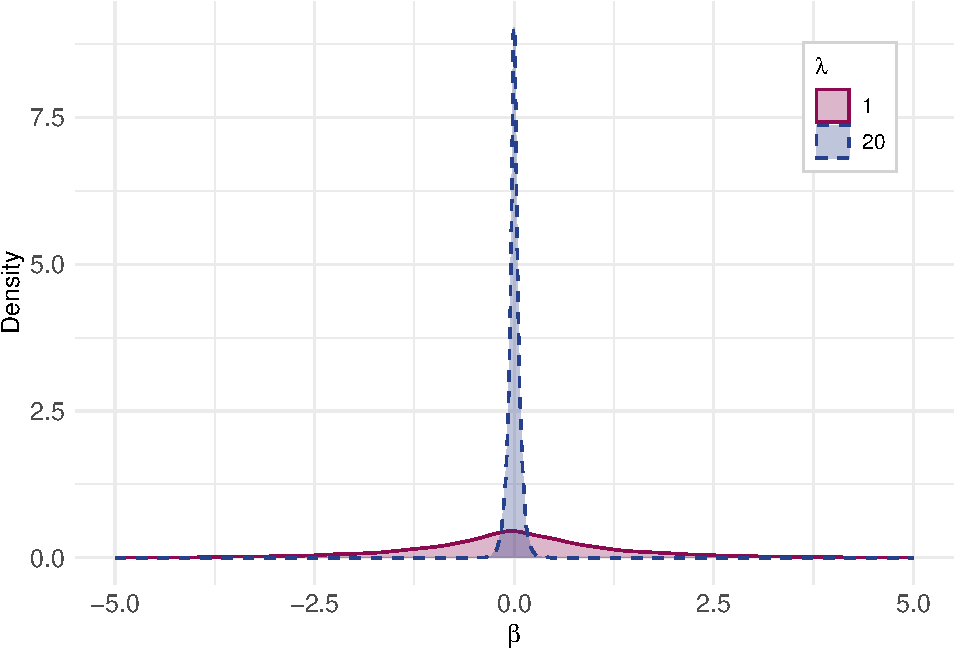
\includegraphics[width=0.75\linewidth]{dissertation_files/figure-latex/SSLASSO Priors-1} 

}

\caption{Density Plots of Laplace Distributions: Impact of Scale Parameter}\label{fig:SSLASSO Priors}
\end{figure}

Setting \(\lambda_1 = \lambda_0\) results in the L1 penalty used in the
LASSO. As \(\lambda_0 \rightarrow \infty\), the spike-and-slab LASSO
approaches the ideal point-mass model. Therefore, the SSL prior allows
for a non-concave continuum between penalised likelihood and point-mass
constructs.

The SSL prior, a mixture of two Laplace distributions, can be viewed as
a two-group refinement of the L1 penalty in LASSO, leading to exactly
sparse posterior modes for \(p(\beta | y)\), enabling simultaneous
variable selection and parameter estimation. This offers an advantage
over traditional spike-and-slab formulations, which often require post
hoc thresholding. Although the original LASSO is known to suffer from
estimation bias, SSL offers two key advantages, as demonstrated by
Tadesse and Vannucci (\protect\hyperlink{ref-Tadesse2022}{2022}). First,
it adaptively mixes two LASSO ``bias'' terms, applying either high
shrinkage for small \(|\beta_i|\) or low shrinkage for large
\(|\beta_i|\). Unlike the adaptive LASSO, which assigns fixed penalties,
SSL adjusts the coefficient-specific penalties to extremes. Second, the
prior on \(\theta\) introduces dependency in the marginal prior
\(p(\beta)\) and non-separability in the SSL penalty, enabling SSL to
borrow information across coordinates and adapt to sparsity information.
The \emph{`SSLASSO'} package fits a set of models, each distinguished by
the regularisation parameter \(\lambda_0\), using a coordinate descent
algorithm. This algorithm utilises screening rules to exclude irrelevant
predictors, adopting a similar approach to that proposed by Breheny
(\protect\hyperlink{ref-Breheny2011}{\textbf{Breheny2011?}}).

\subsubsection{Horseshoe Priors}

The horseshoe prior was introduced by Carvalho, Polson, and Scott
(\protect\hyperlink{ref-Carvalho2009}{\textbf{Carvalho2009?}}), who
characterised it as multivariate-normal scale mixtures. They further
modified the prior specification to set \(\lambda_i\) to be
conditionally independent as further defined
(\protect\hyperlink{ref-Carvalho2010}{Carvalho et al., 2010}). In the
context of a p-dimensional vector
\(y|\theta \sim N(\theta, \sigma^2I)\), when sparsity is assumed for
\(\beta\), the Bayesian horseshoe prior, denoted as \(\pi_{HS}\), is
applied. The assumption here is that each \(\beta_i\) is conditionally
independent, each having a density of \(\pi_{HS} (\beta_i | \tau)\). The
horseshoe prior is then formulated as follows:

\begin{align*}
\beta_i | \lambda_i &\sim \mathcal{N}(0, \lambda_i^2), \quad \text{for } i = 1,\ldots,p, \\
\lambda_i | \tau &\sim \mathcal{C}^+(0, \tau), \\
\tau | \sigma &\sim \mathcal{C}^+(0, \sigma), 
\end{align*}

where \(\mathcal{N}\) is the normal distribution and \(\mathcal{C}^+\)
is the half-Cauchy distribution, specifically over the positive reals
with a scale parameter denoted by \(a\). It is vital to note that each
\(\beta_i\) is a mixture of its own \(\lambda_i\) and that all
\(\lambda_i\) elements have a half-Cauchy prior with a common scale,
\(\tau\). The \(\lambda_i\) is referred to as the local shrinkage
parameter and \(\tau\) as the global shrinkage parameter. Additionally,
Jeffreys' prior is employed for the variance, denoted by
\(p(\sigma^2) \propto 1/\sigma^2\), which is non-informative. Similarly,
the prior for \(\tau\) also follows Jeffreys' treatment, scaled by
\(\sigma\), the standard deviation of the error model.

The horseshoe prior enforces sparsity on the regression coefficients
\(\boldsymbol{\beta}\). Specifically, the posterior mean of each
coefficient \(\beta_j\) can be expressed as a linear function of the
corresponding observation \(y_i\):

\begin{equation}
E(\beta_i|y_i) = y_i(1 - E(k_i|y_i)),
\end{equation}

where \(k_i\) represents the shrinkage coefficient. The half-Cauchy
prior on \(\lambda_i\) induces a Beta\((\frac{1}{2}, \frac{1}{2})\)
distribution for \(k_i\), which has a horseshoe shape. For
\(k_i \approx 0\), there is negligible shrinkage representing signals,
while for \(k_i \approx 1\), there is substantial shrinkage representing
noise.

The horseshoe prior has the property that it tends to shrink the
majority of the coefficients \(\beta_j\) towards zero, enforcing
sparsity, while allowing some coefficients to remain large if they are
indeed associated with the response variable: its flat, Cauchy-like
tails, ensures that significant signals maintain their magnitude,
resulting in minimal post-hoc shrinkage. Simultaneously, its infinitely
tall spike centred at the origin facilitates intense shrinkage for
elements of \(\beta\) that are zero, effectively emphasising the sparse
nature of the solution (\protect\hyperlink{ref-Carvalho2010}{Carvalho et
al., 2010}). A notable advantage of the horseshoe prior is that it does
not require user-specified hyperparameters as the priors for
\(\lambda_i\), \(\tau\), and \(\sigma\) are fully defined. Figure XX
showcases the horseshoe prior with three different magnitudes of the
global shrinkage parameter. As visible from the plot, a smaller \(\tau\)
value tends to concentrate more mass around zero, thereby leading to an
amplified global shrinkage effect.

\begin{figure}

{\centering 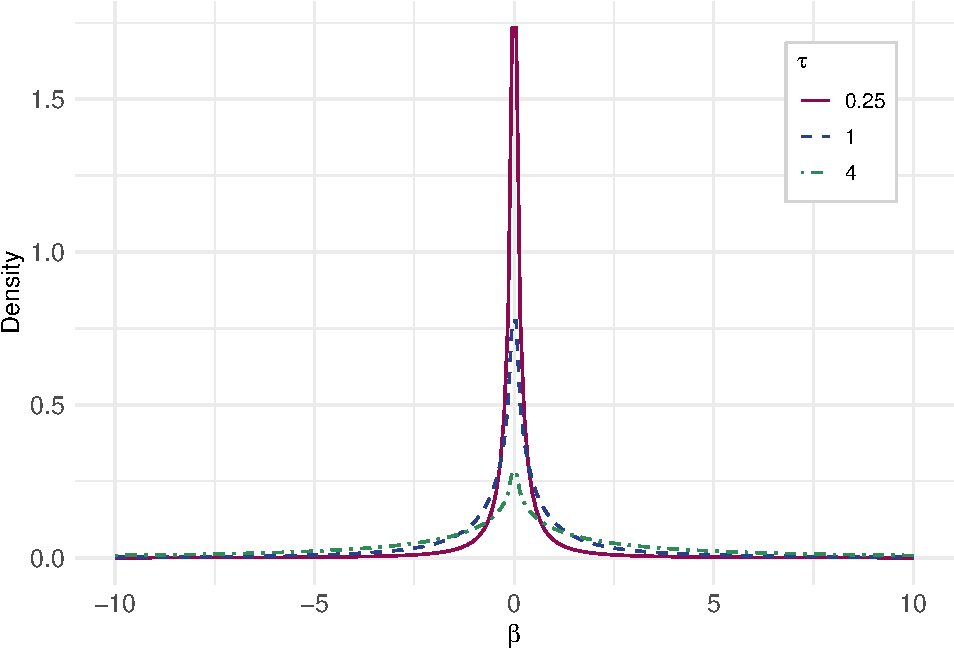
\includegraphics[width=0.75\linewidth]{dissertation_files/figure-latex/Horseshoe Priors-1} 

}

\caption{Density Plots of Horseshoe Distributions: Impact of tau}\label{fig:Horseshoe Priors}
\end{figure}

Horseshoe +

The horseshoe+ estimator
(\protect\hyperlink{ref-Bhadra2016}{\textbf{Bhadra2016?}}), an extension
of the horseshoe estimator, excels in ultra-sparse problems. In contrast
to the horseshoe estimator, the horseshoe+ estimator has a lower
posterior mean squared error and faster posterior concentration rates in
terms of the Kullback--Leibler divergence metric. The prior distribution
\(\pi_{HS+}\) for local shrinkage hyperparameters
\((\lambda_1, . . . , \lambda_p)\) retains the zero-mean half-Cauchy
form and an additional layer of hyperparameters
\((\eta_1, . . . , \eta_p)\) is applied. Each \(\eta_i\) relates to the
prior variance of the corresponding hyperparameter \(\lambda_i\),
creating an expanded hierarchy, as per
(\protect\hyperlink{ref-Makalic2016}{Makalic \& Schmidt, 2016}):

\begin{align}
\beta_i | \lambda_i, \eta_i, \tau &\sim \mathcal{N}(0, \lambda_i^2), \\
\lambda_i | \eta_i, \tau &\sim \mathcal{C}^+(0, \tau \eta_i), \\
\eta_i &\sim \mathcal{C}^+(0,1). \\
\end{align}

In both horseshoe and horseshoe+ models, the local shrinkage random
effects \(\lambda_i\) are not marginally independent after the global
shrinkage parameter \(\tau\) is considered. The horseshoe+ model further
develops the concept by introducing an additional level of local
shrinkage parameters \(\eta_i\) alongside \(\tau\), yielding
conditionally independent \(\lambda_i\). Integrating over \(\eta_i\)
yields \(\lambda_i\)'s density:

\begin{equation}
p(\lambda_i|\tau) = \frac{4 \log(\lambda_i/\tau)}{\pi^2\tau(\lambda_i/\tau)^2 -1} \tag{7}
\end{equation}

The introduction of the additional \(\log(\lambda_i/\tau)\) term in the
numerator leads to unique properties for the proposed estimator. Global
shrinkage parameter \(\tau\) can be handled in various ways. A full
Bayesian approach might involve assigning a standard half-Cauchy or
Uniform(0,1) prior on \(\tau\). An alternative approach could appeal to
an asymptotic argument, suggesting \(\tau\)'s empirical Bayes estimator
be set to \(\hat{\tau} = p_n/n\), where \(p_n\) is the count of non-zero
entries in \(\theta\).

\begin{figure}

{\centering 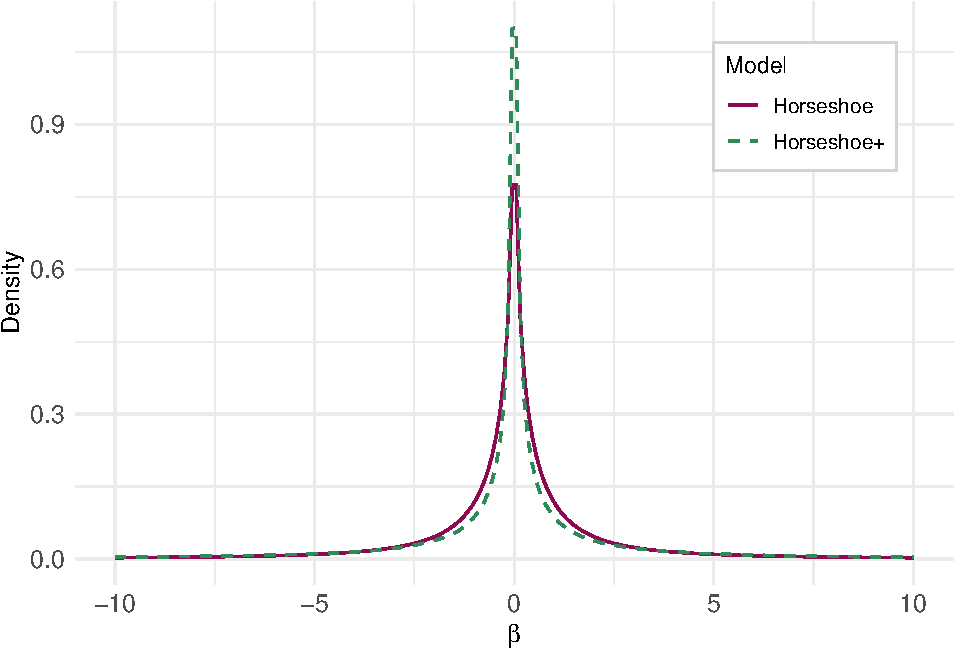
\includegraphics[width=0.75\linewidth]{dissertation_files/figure-latex/Horseshoe Plus Priors-1} 

}

\caption{Density Plots of Horseshoe and Horseshoe+ Prior Distributions}\label{fig:Horseshoe Plus Priors}
\end{figure}

As the usage of Horseshoe prior in Bayesian variable methodology is
prominent, this thesis explores two R packages that employ it, namely
\emph{`bayesreg'} and \emph{' horseshoe'} with some distinct features.

\#Bayesreg package

The \emph{'bayesreg'} package, introduced by Bhattacharya, Chakraborty
and Mallick (\protect\hyperlink{ref-Bhattacharya2016}{2016}), fits
linear or generalised linear regression models using Bayesian
global-local shrinkage prior hierarchies, described by Polson and Scott
(\protect\hyperlink{ref-Polson2010}{Polson \& Scott, 2010}). This thesis
narrows its focus specifically on the horseshoe and horseshoe+, which
are adept at handling high-dimensional datasets. The package
automatically groups factor variables together and applies an additional
level of shrinkage to the set of dummy variables that these factor
variables are expanded into, this is a way to control the complexity of
the model. It also provides both variable ranking and importance,
credible intervals, and diagnostics, which include earlier described
WAIC to assist with prior selection. The \emph{'bayesreg'} package
employs Gibbs sampling for its implementation and strategically selects
between two algorithms for the efficient sampling of regression
coefficients based on the ratio of predictors to sample size: Rue's
algorithm when p/n \textless{} 2 (\protect\hyperlink{ref-Rue2001}{Rue,
2001}), and Bhattacharya et al.'s algorithm otherwise
(\protect\hyperlink{ref-Shin2015}{Shin et al., 2015}). This approach
circumvents the computational and numerical accuracy challenges inherent
in directly computing matrix inverses, particularly in high-dimensional
settings.

\#Horseshoe package

The \emph{`horseshoe'} package allows for conducting sparse linear
regression using the horseshoe prior, providing results such as
posterior means and credible intervals. It is also grounded on the work
of Bhattacharya (\protect\hyperlink{ref-Bhattacharya2016}{2016}). The
package's underlying algorithm updates the global-local scale parameters
through a slice sampling scheme, with the regression coefficients'
posterior samples computed differently depending on whether the number
of predictors is greater or less than/equal to the number of
observations. For the case where \(p > n\), the method proposed by
Bhattacharya et al.
(\protect\hyperlink{ref-Bhattacharya2016}{Bhattacharya et al., 2016}) is
used, while for \(p <= n\), the approach from Rue
(\protect\hyperlink{ref-Rue2001}{Rue, 2001}) is used. Despite not
offering the option to specify the horseshoe+ prior, the package allows
users to select methodological choices for handling the tau and error
variance parameters. For tau, options include ``truncatedCauchy'' for
full Bayes with a truncated Cauchy prior, ``halfCauchy'' for full Bayes
with a half-Cauchy prior, or ``fixed'' for a fixed value approach,
typically based on an empirical Bayes estimate. In this thesis, both are
tested. Regarding the error variance \(\sigma^2\), options include
``Jeffreys'' for full Bayes with Jeffrey's prior or ``fixed'' for a
fixed value, again typically based on an empirical Bayes estimate.

\subsubsection{Shotgun Stochastic Search Algorithm}

On a quest to find a more modern variable selection method within the
Bayesian framework, here is presented the somewhat more recently adapted
version of SSS.

The Shotgun Stochastic Search (SSS) algorithm, introduced by Hans et al.
(\protect\hyperlink{ref-Hans2007}{2007}), is designed to efficiently
navigate high-dimensional model spaces in regression settings with a
large number of candidate predictors, where \(p \gg n\). Its primary
objective is to swiftly pinpoint regions with high posterior
probabilities and ascertain the maximum a posteriori (MAP) model. To
achieve this, the algorithm amalgamates sparsity-inducing priors
promoting parsimony, temperature control akin to that used in global
optimisation algorithms like simulated annealing
(\protect\hyperlink{ref-Vecchi1983}{Kirkpatrick et al., 1983}), and
screening techniques resembling Iterative Sure Independence Screening
(\protect\hyperlink{ref-Fan2008}{Fan \& Lv, 2008}). Furthermore, SSS
exploits parallel computation to enhance performance on cluster
computers.

The MAP model, denoted \(\hat{k}\), is formally defined as:

\begin{equation}
\hat{k} = \underset{k \in \Gamma^*}{\arg\max} \{\pi(k | y)\},
\end{equation}

where \(\Gamma^*\) represents the set of models that are assigned
non-zero prior probability.

In its quest to traverse large model spaces and pinpoint global maxima
efficiently, SSS algorithm defines
\(\text{nbd}(k) = \{\Gamma^+, \Gamma^-, \Gamma^0\}\), where
\(\Gamma^+ = \{k \cup \{j\} : j \in k^c\}\),
\(\Gamma^- = \{k \setminus \{j\} : j \in k\}\), and
\(\Gamma^0 = \{[k \setminus \{j\}] \cup \{l\} : l \in k^c, j \in k\}\).
The \emph{SSS} algorithm proceeds as follows:

\begin{enumerate}
    \item Select an initial model $k^{(1)}$.
    \item For $i = 1$ to $i = N - 1$:
    \begin{itemize}
        \item Compute $\pi(k | y)$ for all $k \in \text{nbd}(k^{(i)})$.
        \item Sample $k^+$, $k^-$, and $k^0$ from $\Gamma^+$, $\Gamma^-$, and $\Gamma^0$, 
        respectively, with probabilities proportional to $\pi(k | y)$.
        \item Sample $k^{(i+1)}$ from $\{k^+, k^-, k^0\}$, with probability proportional to $\{\pi(k^+ | y), \pi(k^- | y), \pi(k^0 | y)\}$.
    \end{itemize}
\end{enumerate}

The MAP model is determined as the model with the highest unnormalised
posterior probability among those models searched by SSS.

\emph{S5}

As the objective of this thesis is to blend statistical methodology with
application, it is imperative to dissect the proposed computational
tools. Over the years, the SSS algorithm has evolved, and a streamlined
version incorporating screening has been developed and made available
through the package Bayes5 (\protect\hyperlink{ref-Shin2015}{Shin et
al., 2015}).

The Simplified Shotgun Stochastic Search with Screening (S5) algorithm
is a modified version of the SSS designed to further enhance
computational efficiency. S5 restricts its search to models in
\(\Gamma^+\) and \(\Gamma^-\), thereby omitting the computationally
intensive evaluation of marginal probabilities for models in
\(\Gamma^0\). However, this focused search might lead the algorithm to
overlook certain high-posterior probability regions and risk settling in
local maxima. To mitigate this, S5 introduces a temperature parameter,
akin to simulated annealing, enabling broader exploration.

Furthermore, S5 incorporates an Iterative Sure Independence Screening
strategy to focus on variables highly correlated with the residuals of
the current model. Specifically, it assesses \(|r_k^T X_j|\), where
\(r_k\) is the residual of model \(k\), for \(j = 1, \ldots, p\), and
prioritises variables for which this product is large.

In S5, \(S_k\) represents the union of variables in \(k\) and the top
\(M_n\) variables obtained through residual-based screening. The
screened neighborhood, denoted as
\(\text{nbd}_{scr}(k) = \{\Gamma^{+}_{\text{scr}}, \Gamma^{-}\}\), is
defined with
\(\Gamma^{+}_{\text{scr}} = \{k \cup \{j\} : j \in k^c \cap S_k\}\).
This results in a scalable algorithm, particularly beneficial when the
number of variables \(p\) is large.

S5 algorithm employs a temperature schedule and utilises a screened set
of variables to improve efficiency in identifying the MAP model. It
approximates the posterior model probability and assesses model space
uncertainty by approximating the normalising constant from the
unnormalised posterior probabilities.

The computational complexity of the original SSS algorithm is
proportional to the product of the number of models explored and the
complexity of evaluating the unnormalised posterior probability for the
largest model, denoted as \(E_n\), and is given by
\([ O\{Np\} + O\{Nq_n\} + O\{N(p-q_n)q_n\} ] \times E_n\), where \(q_n\)
is the maximum size of model among searched models and \(q_n < n <<p\).

In contrast, S5 dramatically reduces the number of models considered by
focusing on \(M_n\) variables post-screening. This leads to a
computational complexity of
\([O\{JL(M_n - q_n)\} + O(JLM_n)] \times E_n + O(JLnp)\), where
\(q_n < M_n\). The algorithm is scalable since its complexity is
relatively insensitive to the size of \(p\).

Shin et al. (\protect\hyperlink{ref-Shin2015}{2015}) demonstrated that
S5 is significantly faster than SSS in identifying the MAP model and
requires fewer model evaluations.

\newpage

\section{Simulated Data Study}

\subsection{Simulation Overview}

As noted before, variable selection methods are applied within the
framework of linear regression, denoted by \(Y = X\beta + e\), where
\(e \sim \mathcal{N}(0, \sigma^2)\). The thesis provides an analytical
contrast between Bayesian techniques and their frequentist counterparts,
specifically, Lasso and Elastic Net penalisations, which were rigorously
studied in semesters 1 and 2. Additionally, a contemporary machine
learning technique, \emph{XGBoost}, is also applied to provide a
comprehensive comparative.

Each of the datasets \emph{Type 1}, \emph{Type 2}, \emph{Type 3}, and
\emph{Type 4} that follow are designed to be adaptable across various
dimensionality settings. To further note, the selection of true signals,
the predetermined magnitude of error variance, and the inclusion of
interaction terms, polynomials, and other features are strategically
chosen to present varying levels of complexity for the models being
tested, thereby examining their robustness and adaptability under
distinct circumstances.

\hfill\break
\hfill\break

The \emph{Type 1} datasets consist of uncorrelated continuous covariates
with a moderate level of noise. The covariates are simulated from a
multivariate normal distribution:

\begin{equation}
\mathbf{X} \sim \text{MVN}(\mathbf{u}_x, \sigma_x^2 \mathbf{\Sigma}_x),
\end{equation}

where \(\mathbf{u}_x\) is a \(1 \times p\) mean vector,
\(\mathbf{\Sigma}_x\) is a \(p \times p\) correlation matrix, and
\(\sigma_x^2\) is the common variance of all covariates. Each \(x_i\) is
normally distributed with a mean of 5, i.e.,
\(\mathbf{u}_x = (5, 5, \ldots, 5)\). \(\mathbf{\Sigma}_x\) is a
\(p \times p\) identity matrix and \(\sigma_x^2 = 1\). The response
variable \(y\) is generated as:

\begin{equation}
\mathbf{y} = \mathbf{X}\boldsymbol{\beta} + \boldsymbol{\epsilon},
\end{equation}

where \(\boldsymbol{\epsilon_i} \sim N(0, \sigma_e^2)\) for
\(i = 1, 2, \ldots, n\). \(\boldsymbol{\beta}\) is a \(p \times 1\)
vector of true coefficients, \(\boldsymbol{\epsilon}\) is an
\(n \times 1\) vector of error terms, \(\sigma_e^2\) is the error
variance, and \(\mathbf{I_n}\) is an \(n \times n\) identity matrix. The
regression coefficients are enforced as
\(\beta_1, \ldots, \beta_{10} = 3\);
\(\beta_{11}, \ldots, \beta_{20} = 5\), and \(\beta_{p-20} = 0\). The
intercept term is zero, and the errors (unexplained variability in the
response variable) are normally distributed with \(\sigma_e^2 = 15\).

\hfill\break
\hfill\break

The \emph{Type 2} dataset comprises continuous covariates with temporal
correlation and moderate noise. The generation of the \emph{Type 2}
dataset parallels the method utilised for the \emph{Type 1} dataset with
certain distinctions. Specifically, the mean vector for the covariates
\(\mathbf{u}_x\) is constructed such that the first 30 variables each
have a mean of 3, and the rest have a mean of 7; that is,
\(\mathbf{u}_x = (3, 3, \ldots, 3, 7, 7, \ldots, 7)\). The covariance
matrix of the covariates \(\mathbf{\Sigma}_x\) adheres to an
autoregressive order 1, commonly refered to as AR(1), structure, with
the correlation coefficient \(\rho = 0.8\), \(\sigma_x^2\) is held
constant at 1. For the response variable, 20 covariates are true
signals. The vector of true regression coefficients,
\(\boldsymbol{\beta}\), is defined with non-zero values for the first 20
entries (e.g., 5 for each), while the remaining entries are set to zero;
thus, \(\boldsymbol{\beta} = (5, 5, \ldots, 5, 0, 0, \ldots, 0)^T\). The
error term variance \(\sigma_e^2 = 10\).

\hfill\break
\hfill\break

The \emph{Type 3} dataset is a rich blend of continuous and categorical
covariates, including interaction terms and polynomial features, with
moderate noise. In this setup, the mean vector for continuous covariates
\(\mathbf{u}_x\) is segmented into three groups: the first 20 variables
have a mean of 2, the next 30 have a mean of 5, and the remaining
variables have a mean of 8, resulting in
\(\mathbf{u}_x = (2, 2, \ldots, 2, 5, 5, \ldots, 5, 8, 8, \ldots, 8)\).
The covariance matrix \(\mathbf{\Sigma}_x\) adheres to an AR(1)
structure with a correlation coefficient of \(\rho = 0.6\), while
\(\sigma_x^2\) remains constant at 1. The vector of true regression
coefficients for continuous predictors, \(\boldsymbol{\beta}\), takes on
values such as
\(\boldsymbol{\beta} = (6, 6, 6, 6, 6, 4, 4, 4, 4, 4, 3, 3, 3, 3, 3, 0, 0, \ldots, 0)^T\).

First categorical variable is binary (akin to having or not having a
certain illness) and is set to have \(\beta = 4\). Second categorical
variable is treated as ordinal, with categories 1 through 5 (serves as
ordered category, f.e., progressive education levels from middle school
to higher degree) and is set to have \(\beta = 0\).

Interaction terms are created by multiplying selected pairs of
covariates: \(X1\) and \(X2\) continuous, \(X3\) and \(X4\) continuous,
\(X11\) and \(X22\) continuous, \(binary categorical\) and \(X22\)
continuous. Polynomial features are generated by elevating \(X5\) and
\(X23\) covariates to the power of 2, and \(X6\), \(X23\) to the power
of 3. From interaction terms and polynomials, only \(X1 : X2\) was
enforced to have \(\beta = 3\) and \(X23^2\) to have \(\beta = 6\), the
rest have \(\boldsymbol{beta} = (0, \ldots, 0)\)

The intercept, in this context, has set to a of value 2, serving as the
expected response value when all covariates are at zero. Lastly, the
error term variance is set at \(\sigma_e^2 = 12\).

\hfill\break
\hfill\break

The \emph{Type 4} dataset is characterised by grouping structures among
continuous covariates, where covariates within each group are highly
correlated, while covariates between different groups are independent.
The mean vector for continuous covariates \(\mathbf{u}_x\) is segmented
into five groups,
i.e.~\(\mathbf{u}_x = (2, \ldots, 2, 4, \ldots, 4, 6, \ldots, 6, 8 \ldots, 8, 10, \ldots, 10)\).
The vector of true regression coefficients corresponding to true signals
within each group
\(\boldsymbol{\beta} = (6, 6, 6, 6, 6, 4, 4, 4, 4, 4, 3, 3, 3, 3, 3, 0, \ldots, 0)^T\),
where the number of groups \(T = 5\).

The covariance matrix \(\mathbf{\Sigma}_x\) is constructed as a
block-diagonal matrix, where each block corresponds to a group, and
within each block, the elements are highly correlated. The diagonal
blocks can have a specific structure, the AR(1), with correlation
coefficients \(\rho = 0.6\), while the off-diagonal blocks are matrices
of zeros, indicating independence between groups.

First categorical variable is binary and is set to have \(\beta = 4\).
Second categorical variable is treated as ordinal, with categories 1
through 5 and is set to have \(\beta = 0\). Interaction terms are
created by multiplying selected covariates: the continuous \(X1\),
\(X2\) and \(X3\), \(X3\) and \(X4\), \(X16\) and \(X17\). \(X1:X2:X3\)
was enforced to have \(\beta = 3\), \(X4 : X5\) and \(X16 : X17\) to
have \(\beta = 0\). The error term variance is set at
\(\sigma_e^2 = 10\).

Four different dimensionality settings are considered under all four
data types: \(p(50) < n(200)\), reflecting a traditional setting with
more observations than variables; \(p(100) = n(100)\), representing a
balanced case; \(p(200) > n(150)\), indicative of high-dimensional
scenarios such as in genomics; and \(p(200) \gg n(50)\), where the
number of variables substantially surpasses the number of observations.
An additional configuration is proposed to better suit \emph{XGBoost's}
strengths and establish a baseline performance capacity. While retaining
the data generation methodology outlined earlier, a subsequent dataset
is simulated with a modified proportion of data points to features,
namely \(p=50, n=500\). These settings enable comparisons within data
types and offer insights into practical challenges regarding data
availability and computation. The choice of \(p\) and \(n\) values is
guided by computation time and an approximation to real-world data,
where obtaining data can be costly. This structure facilitates a
comprehensive analysis of various scenarios. For reference, for all data
generation the reproducibility seed was set to \(42\).

\subsection{Type 1}

XGBoost selection of variables requires to set a threshold. For feature
importance list with weights, see Appendix XX.

Add results of ceofficients and list which methods do not draw
coefficients to exactly zero. Which methods include confidence intervals
and where is 0 included should be disregarded.

\begin{table}[!h]

\caption{\label{tab:Results T1}Summary of Type 1 Data Results}
\centering
\fontsize{8.5}{10.5}\selectfont
\begin{tabular}[t]{>{}l|>{}l|>{}l|>{}l|>{}l|>{}l|>{}l|>{}l|>{}l|>{}l|>{}l|>{}l|>{}l|>{}l|>{}l|>{}l|>{}l|}
\toprule
\multicolumn{2}{c}{ } & \multicolumn{4}{c}{p < n} & \multicolumn{4}{c}{p = n} & \multicolumn{3}{c}{p > n} & \multicolumn{4}{c}{p >> n} \\
\cmidrule(l{3pt}r{3pt}){3-6} \cmidrule(l{3pt}r{3pt}){7-10} \cmidrule(l{3pt}r{3pt}){11-13} \cmidrule(l{3pt}r{3pt}){14-17}
Package & Method & TS & FP & FN &  & TS & FP & FN &  & TS & FP & FN &  & TS & FP & FN\\
\midrule
\addlinespace[0.3em]
\multicolumn{17}{l}{\textbf{Frequentist Methods}}\\
\hspace{1em}glmnet & LASSO & 20 & 19 & 0 &  & 20 & 50 & 0 &  & 20 & 37 & 0 &  & 10 & 22 & 10\\
\hspace{1em}glmnet & Elastic Net & 20 & 12 & 0 &  & 20 & 37 & 0 &  & 20 & 10 & 0 &  & 12 & 18 & 8\\
\addlinespace[0.3em]
\multicolumn{17}{l}{\textbf{Bayesian Methods}}\\
\hspace{1em}spikeslab & Spike-and-Slab Prior & 20 & 20 & 0 &  & 20 & 79 & 0 &  & 20 & 117 & 0 &  & 12 & 12 & 8\\
\hspace{1em}SSLASSO & Spike-and-Slab LASSO & 20 & 1 & 0 &  & 15 & 5 & 5 &  & 6 & 5 & 14 &  & 20 & 0 & 0\\
\hspace{1em}horseshoe & Horseshoe Prior, TC & 20 & 0 & 0 &  & 20 & 1 & 0 &  & 20 & 0 & 0 &  & 1 & 0 & 19\\
\hspace{1em}horseshoe & Horseshoe Prior, HC & 20 & 0 & 0 &  & 20 & 1 & 0 &  & 20 & 0 & 0 &  & 0 & 0 & 20\\
\hspace{1em}bayesreg & Horseshoe Prior & 20 & 0 & 0 &  & 20 & 1 & 0 &  & 20 & 0 & 0 &  & 7 & 5 & 13\\
\hspace{1em}bayesreg & Horseshoe+ Prior & 20 & 0 & 0 &  & 20 & 1 & 0 &  & 20 & 0 & 0 &  & 8 & 5 & 12\\
\hspace{1em}BayesS5 & S5 Method &  &  &  &  &  &  &  &  &  &  &  &  &  &  & \\
\hspace{1em}monomvn & Bayesian LASSO &  &  &  &  &  &  &  &  &  &  &  &  &  &  & \\
\bottomrule
\multicolumn{17}{l}{\textsuperscript{a} TS=True Signal, FP=False Positive, FN=False Negative}\\
\multicolumn{17}{l}{\textsuperscript{b} p(50) < n(200), p(100) = n(100), p(200) > n(150), p(200) >> n(50)}\\
\end{tabular}
\end{table}

\begin{table}[!h]

\caption{\label{tab:Results XGBoost}Summary of XGBoost Results for All Simulated Data}
\centering
\fontsize{8.5}{10.5}\selectfont
\begin{tabular}[t]{>{}l|>{}l|>{}l|>{}l|>{}l|>{}l|>{}l|>{}l|>{}l|>{}l|>{}l|>{}l|>{}l|>{}l|>{}l|>{}l|>{}l|>{}l|>{}l|>{}l|}
\toprule
\multicolumn{1}{c}{ } & \multicolumn{4}{c}{p << n} & \multicolumn{4}{c}{p < n} & \multicolumn{4}{c}{p = n} & \multicolumn{3}{c}{p > n} & \multicolumn{4}{c}{p >> n} \\
\cmidrule(l{3pt}r{3pt}){2-5} \cmidrule(l{3pt}r{3pt}){6-9} \cmidrule(l{3pt}r{3pt}){10-13} \cmidrule(l{3pt}r{3pt}){14-16} \cmidrule(l{3pt}r{3pt}){17-20}
Data & TS & FP & FN &  & TS & FP & FN &  & TS & FP & FN &  & TS & FP & FN &  & TS & FP & FN\\
\midrule
Type 1 &  &  &  &  &  &  &  &  &  &  &  &  &  &  &  &  &  &  & \\
Type 2 &  &  &  &  &  &  &  &  &  &  &  &  &  &  &  &  &  &  & \\
Type 3 &  &  &  &  &  &  &  &  &  &  &  &  &  &  &  &  &  &  & \\
Type 4 &  &  &  &  &  &  &  &  &  &  &  &  &  &  &  &  &  &  & \\
Type 5 &  &  &  &  &  &  &  &  &  &  &  &  &  &  &  &  &  &  & \\
\bottomrule
\multicolumn{20}{l}{\textsuperscript{a} TS=True Signal, FP=False Positive, FN=False Negative}\\
\multicolumn{20}{l}{\textsuperscript{b} p(50) << n(500), p(50) < n(200), p(100) = n(100), p(200) > n(150), p(200) >> n(50)}\\
\end{tabular}
\end{table}

\subsection{Type 2}

Bla bla

\begin{table}[!h]

\caption{\label{tab:Results T2}Summary of Type 2 Data Results}
\centering
\fontsize{8.5}{10.5}\selectfont
\begin{tabular}[t]{>{}l|>{}l|>{}l|>{}l|>{}l|>{}l|>{}l|>{}l|>{}l|>{}l|>{}l|>{}l|>{}l|>{}l|>{}l|>{}l|>{}l|}
\toprule
\multicolumn{2}{c}{ } & \multicolumn{4}{c}{p < n} & \multicolumn{4}{c}{p = n} & \multicolumn{3}{c}{p > n} & \multicolumn{4}{c}{p >> n} \\
\cmidrule(l{3pt}r{3pt}){3-6} \cmidrule(l{3pt}r{3pt}){7-10} \cmidrule(l{3pt}r{3pt}){11-13} \cmidrule(l{3pt}r{3pt}){14-17}
Package & Method & TS & FP & FN &  & TS & FP & FN &  & TS & FP & FN &  & TS & FP & FN\\
\midrule
\addlinespace[0.3em]
\multicolumn{17}{l}{\textbf{Frequentist Methods}}\\
\hspace{1em}glmnet & LASSO & 20 & 0 & 0 &  & 20 & 9 & 0 &  & 20 & 6 & 0 &  & 20 & 7 & 0\\
\hspace{1em}glmnet & Elastic Net & 20 & 0 & 0 &  & 20 & 0 & 0 &  & 20 & 0 & 0 &  & 20 & 2 & 0\\
\addlinespace[0.3em]
\multicolumn{17}{l}{\textbf{Bayesian Methods}}\\
\hspace{1em}spikeslab & Spike-and-Slab Prior & 20 & 2 & 0 &  & 20 & 75 & 0 &  & 20 & 8 & 0 &  & 20 & 25 & 0\\
\hspace{1em}SSLASSO & Spike-and-Slab LASSO & 17 & 0 & 3 &  & 8 & 0 & 12 &  & 1 & 0 & 19 &  & 13 & 0 & 7\\
\hspace{1em}horseshoe & Horseshoe Prior, TC & 20 & 0 & 0 &  & 20 & 2 & 0 &  & 20 & 0 & 0 &  & 3 & 0 & 17\\
\hspace{1em}horseshoe & Horseshoe Prior, HC & 20 & 0 & 0 &  & 20 & 1 & 0 &  & 20 & 0 & 0 &  & 2 & 0 & 18\\
\hspace{1em}bayesreg & Horseshoe Prior & 20 & 0 & 0 &  & 20 & 2 & 0 &  & 20 & 0 & 0 &  & 18 & 0 & 2\\
\hspace{1em}bayesreg & Horseshoe+ Prior & 20 & 0 & 0 &  & 20 & 2 & 0 &  & 20 & 0 & 0 &  & 20 & 0 & 0\\
\hspace{1em}BayesS5 & S5 Method &  &  &  &  &  &  &  &  &  &  &  &  &  &  & \\
\hspace{1em}monomvn & Bayesian LASSO &  &  &  &  &  &  &  &  &  &  &  &  &  &  & \\
\bottomrule
\multicolumn{17}{l}{\textsuperscript{a} TS=True Signal, FP=False Positive, FN=False Negative}\\
\multicolumn{17}{l}{\textsuperscript{b} p(50) < n(200), p(100) = n(100), p(200) > n(150), p(200) >> n(50)}\\
\end{tabular}
\end{table}

\subsection{Type 3}

Bla bla

\begin{table}[!h]

\caption{\label{tab:Results T3}Summary of Type 3 Data Results}
\centering
\fontsize{8.5}{10.5}\selectfont
\begin{tabular}[t]{>{}l|>{}l|>{}l|>{}l|>{}l|>{}l|>{}l|>{}l|>{}l|>{}l|>{}l|>{}l|>{}l|>{}l|>{}l|>{}l|>{}l|}
\toprule
\multicolumn{2}{c}{ } & \multicolumn{4}{c}{p < n} & \multicolumn{4}{c}{p = n} & \multicolumn{3}{c}{p > n} & \multicolumn{4}{c}{p >> n} \\
\cmidrule(l{3pt}r{3pt}){3-6} \cmidrule(l{3pt}r{3pt}){7-10} \cmidrule(l{3pt}r{3pt}){11-13} \cmidrule(l{3pt}r{3pt}){14-17}
Package & Method & TS & FP & FN &  & TS & FP & FN &  & TS & FP & FN &  & TS & FP & FN\\
\midrule
\addlinespace[0.3em]
\multicolumn{17}{l}{\textbf{Frequentist Methods}}\\
\hspace{1em}glmnet & LASSO & 18 & 11 & 0 &  & 18 & 13 & 0 &  & 18 & 10 & 0 &  & 17 & 14 & 1\\
\hspace{1em}glmnet & Elastic Net & 18 & 6 & 0 &  & 17 & 6 & 1 &  & 18 & 2 & 0 &  & 15 & 6 & 3\\
\addlinespace[0.3em]
\multicolumn{17}{l}{\textbf{Bayesian Methods}}\\
\hspace{1em}spikeslab & Spike-and-Slab Prior & 17 & 10 & 1 &  & 18 & 82 & 0 &  & 18 & 19 & 0 &  & 9 & 36 & 9\\
\hspace{1em}SSLASSO & Spike-and-Slab LASSO & 18 & 4 & 0 &  & 12 & 2 & 6 &  & 16 & 1 & 2 &  & 4 & 1 & 14\\
\hspace{1em}horseshoe & Horseshoe Prior, TC & 17 & 0 & 1 &  & 17 & 0 & 1 &  & 17 & 0 & 1 &  & 5 & 2 & 12\\
\hspace{1em}horseshoe & Horseshoe Prior, HC & 17 & 0 & 1 &  & 17 & 0 & 1 &  & 17 & 0 & 1 &  & 5 & 1 & 12\\
\hspace{1em}bayesreg & Horseshoe Prior & 18 & 1 & 0 &  & 18 & 1 & 0 &  & 18 & 1 & 0 &  & 0 & 0 & 0\\
\hspace{1em}bayesreg & Horseshoe+ Prior & 18 & 0 & 0 &  & 18 & 2 & 0 &  & 18 & 0 & 0 &  & 10 & 5 & 8\\
\hspace{1em}BayesS5 & S5 Method &  &  &  &  &  &  &  &  &  &  &  &  &  &  & \\
\hspace{1em}monomvn & Bayesian LASSO &  &  &  &  &  &  &  &  &  &  &  &  &  &  & \\
\bottomrule
\multicolumn{17}{l}{\textsuperscript{a} TS=True Signal, FP=False Positive, FN=False Negative}\\
\multicolumn{17}{l}{\textsuperscript{b} p(50) < n(200), p(100) = n(100), p(200) > n(150), p(200) >> n(50)}\\
\end{tabular}
\end{table}

\subsection{Type 4}

Bla bla

\begin{table}[!h]

\caption{\label{tab:Results T4}Summary of Type 4 Data Results}
\centering
\fontsize{8.5}{10.5}\selectfont
\begin{tabular}[t]{>{}l|>{}l|>{}l|>{}l|>{}l|>{}l|>{}l|>{}l|>{}l|>{}l|>{}l|>{}l|>{}l|>{}l|>{}l|>{}l|>{}l|}
\toprule
\multicolumn{2}{c}{ } & \multicolumn{4}{c}{p < n} & \multicolumn{4}{c}{p = n} & \multicolumn{3}{c}{p > n} & \multicolumn{4}{c}{p >> n} \\
\cmidrule(l{3pt}r{3pt}){3-6} \cmidrule(l{3pt}r{3pt}){7-10} \cmidrule(l{3pt}r{3pt}){11-13} \cmidrule(l{3pt}r{3pt}){14-17}
Package & Method & TS & FP & FN &  & TS & FP & FN &  & TS & FP & FN &  & TS & FP & FN\\
\midrule
\addlinespace[0.3em]
\multicolumn{17}{l}{\textbf{Frequentist Methods}}\\
\hspace{1em}glmnet & LASSO & 17 & 10 & 0 &  & 17 & 3 & 0 &  & 17 & 6 & 0 &  & 16 & 9 & 1\\
\hspace{1em}glmnet & Elastic Net & 17 & 3 & 0 &  & 17 & 2 & 0 &  & 16 & 5 & 1 &  & 16 & 10 & 1\\
\addlinespace[0.3em]
\multicolumn{17}{l}{\textbf{Bayesian Methods}}\\
\hspace{1em}spikeslab & Spike-and-Slab Prior & 17 & 7 & 0 &  & 17 & 77 & 0 &  & 17 & 47 & 0 &  & 16 & 27 & 1\\
\hspace{1em}SSLASSO & Spike-and-Slab LASSO & 15 & 5 & 2 &  & 8 & 2 & 9 &  & 12 & 4 & 5 &  & 1 & 0 & 16\\
\hspace{1em}horseshoe & Horseshoe Prior, TC & 16 & 0 & 1 &  & 16 & 0 & 1 &  & 16 & 0 & 1 &  & 2 & 0 & 15\\
\hspace{1em}horseshoe & Horseshoe Prior, HC & 16 & 0 & 1 &  & 16 & 0 & 1 &  & 16 & 0 & 1 &  & 2 & 0 & 15\\
\hspace{1em}bayesreg & Horseshoe Prior & 17 & 0 & 0 &  & 17 & 0 & 0 &  & 17 & 0 & 0 &  & 14 & 6 & 3\\
\hspace{1em}bayesreg & Horseshoe+ Prior & 17 & 0 & 0 &  & 17 & 0 & 0 &  & 17 & 0 & 0 &  & 13 & 4 & 4\\
\hspace{1em}BayesS5 & S5 Method &  &  &  &  &  &  &  &  &  &  &  &  &  &  & \\
\hspace{1em}monomvn & Bayesian LASSO &  &  &  &  &  &  &  &  &  &  &  &  &  &  & \\
\bottomrule
\multicolumn{17}{l}{\textsuperscript{a} TS=True Signal, FP=False Positive, FN=False Negative}\\
\multicolumn{17}{l}{\textsuperscript{b} p(50) < n(200), p(100) = n(100), p(200) > n(150), p(200) >> n(50)}\\
\end{tabular}
\end{table}

\subsection{Discussion}

Bla bla bla

\newpage

\section{Crime Data}

While the analysis of simulated data establishes a foundational
understanding of various methodologies in a controlled environment, it
is vital to extend this analysis to a real data set. Real data often
present a more complex set of challenges and intricacies. Due to
personal interest, the data set chosen is regarding sociological issues.

The dataset under study amalgamates socio-economic data from the 1990
Census, law enforcement data from the 1990 Law Enforcement Management
and Admin Stats survey, and crime data from the 1995 Federal Bureau of
Investigation Uniform Crime Reports (FBI UCR) for various communities in
the U.S. Comprising 2215 instances and 147 attributes, the dataset
includes factors related to community characteristics, law enforcement,
and crime rates, focusing on 125 predictive attributes and 18 potential
target variables (crime attributes). It is essential to recognise that
the dataset has limitations due to discrepancies in population values,
the omission of some communities, and the absence of certain data,
particularly regarding rapes. The FBI cautions against using this
dataset as the sole criterion for evaluating communities, as it does not
encompass all relevant factors. For a comprehensive list of variables
included in the dataset, please refer to Appendix Table XX.

The wrangled data consist of 99 variables: 98 predictors and the target
variable ``Violent Crimes per 100k Population'' with 1992 instances. The
other variables were disregarded as community names were non-predictive.
Additionally, the analysis disregarded variables with over 80\% missing
values to maintain data integrity and reliable outputs. The data set was
donated to UC Irvine Machine Learning Repository and is accessible
online. For a more comprehensive understanding, refer to UC Irvine
Machine Learning Repository
(\protect\hyperlink{ref-misc_communities_and_crime_unnormalized_211}{Redmond,
2011}).

\subsection{Ethical Considerations}

Algorithmic decision-making mechanisms permeate many sectors of modern
life, from spam classification in emails to credit scoring and
employment candidate assessment. However, concerns have emerged
regarding transparency, accountability, and fairness, specifically when
these systems predicate their decisions on historical data. There exists
a risk of perpetuating biases against certain demographic groups
identified by ``sensitive attributes'', such as gender, age, race, or
religion, should these groups have been historically correlated with
higher risk factors (\protect\hyperlink{ref-Komiyama2018}{Komiyama et
al., 2018}). Such variables refer to data that could be used to predict
attributes protected by anti-discrimination laws, where the prejudiced
actions are directed towards individuals based on their membership in
certain groups, rather than assessing them on their individual merits.
The caution around discriminatory impacts can manifest in two
significant forms: disparate treatment and disparate impact
(\protect\hyperlink{ref-Zafar2017}{Zafar et al., 2017}). The former
describes intentional discrimination against groups with evidence of
explicit reference to group membership. The latter examines the
unintentional yet potentially harmful consequences that decision-making
processes can have on specific groups, and despite it being facially
neutral, it can still contribute to unintentional discrimination.

Decision-making entities such as banks, consultancies, and universities
must strive to build classifiers free from discrimination, even if their
historical data might inherently contain discriminatory elements.
Žliobaitė et al. (\protect\hyperlink{ref-Zliobaite2011}{2011}) highlight
a legal case where a leading consultancy firm faced allegations of
indirect racial discrimination. They used existing criminal records for
pre-employment screening, inadvertently creating bias because of the
data's historical correlation between race and criminality. Even though
the firm did not intend to discriminate, its use of criminal records
resulted in racial discrimination. This case underscores that
discrimination can inadvertently occur, even when sensitive information
is not explicitly employed in the model, and such indirect
discrimination is also legally unacceptable.

Likewise, Komiyama et al. (\protect\hyperlink{ref-Komiyama2018}{2018})
has pointed out that the mere exclusion of the ``sensitive variables''
is not sufficient. The publication further proposed the fairness of an
algorithm through a coefficient of determination (CoD) of the sensitive
attributes as a constraint. The CoD measures the predictable proportion
of the variance of an estimator from sensitive attributes, effectively
extending the correlation coefficient for multiple sensitive
characteristics. For a deeper exploration of this topic, particularly in
the realms of linear and logistic regression, readers are directed to
the works of (\protect\hyperlink{ref-Scutari2022}{Scutari et al.,
2022}), (\protect\hyperlink{ref-Komiyama2018}{Komiyama et al., 2018}),
and (\protect\hyperlink{ref-Zliobaite2011}{Žliobaitė et al., 2011}).

In this thesis, the pre-selection of variables included a thoughtful
consideration of data sensitivity. The crime data used here include the
variables describing the percentage of the African American population
and the percentage of foreign-born individuals. Though a more in-depth
exploration of sensitivity could be a progressive step beyond this work,
it was deemed pertinent to acknowledge ongoing developments in data
decision methodologies in ethically charged contexts. Thus, this thesis
pivots back to the exclusion of the aforementioned variables,
particularly those that could raise potential legal and ethical concerns
in the application of the final model. Furthermore, the analysis
explores interactions between variables to uncover potential underlying
complex relationships. This approach aims to commit to bias prevention
and the promotion of ethical data analysis.

\subsection{Exploratory Data Analysis}

Before proceeding with model fitting, conducting exploratory data
analysis is standard statistical practice, it is important to spot any
unwanted data characteristics that could adversely impact the models.

Firstly, to apply linear regression, it is vital to assess the normality
assumption underlying it. The Shapiro-Wilk Normality test yields
p-values well below \(0.05\) for all variables, providing evidence to
reject the normality hypothesis. Given the skewness in most variables'
distribution, illustrated by the sample histogram in \(Figure XX\), a
\(log(X + 1)\) transformation is applied across all variables. While
this aids in normalising the data, it also complicates the
interpretation of variable importance later. Post-transformation, the
Normality test shows marginal improvement but still falls short of
confirming normal distribution for all variables, see \(Figure XX\).

\begin{figure}[H]

{\centering 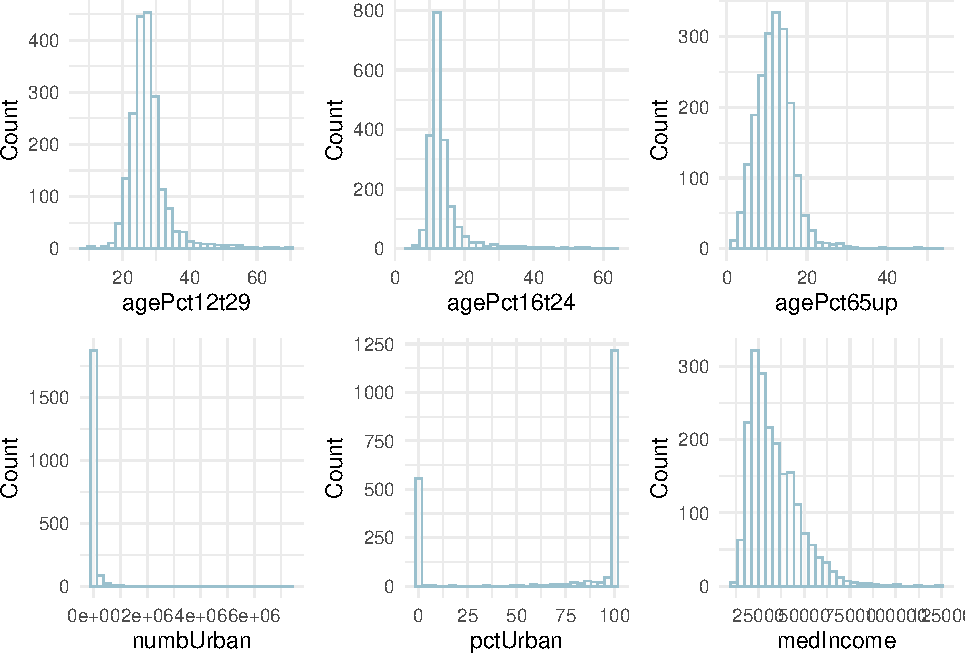
\includegraphics[width=0.85\linewidth]{dissertation_files/figure-latex/Histograms df Plot-1} 

}

\caption{Crime Data: Sample Histograms Illustrating Variable Distribution Prior to Transformation}\label{fig:Histograms df Plot}
\end{figure}

\begin{figure}[H]

{\centering 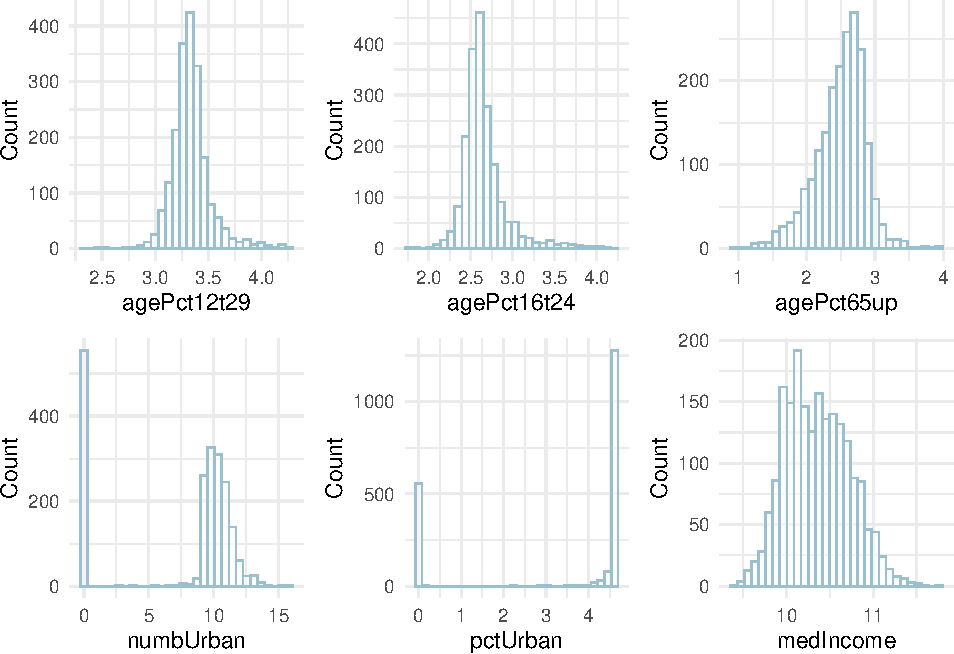
\includegraphics[width=0.85\linewidth]{dissertation_files/figure-latex/Histograms df_t Plot-1} 

}

\caption{Crime Data: Sample Histograms Demonstrating Variable Distribution Post Logarithmic Transformation}\label{fig:Histograms df_t Plot}
\end{figure}

Addressing outliers is typically critical since they can influence model
performance and alter the correlations between variables. Tukey's
approach to spotting high outliers in data variables, as described in
Kannan et al. (\protect\hyperlink{ref-Kannan2015}{2015}), entails
determining the interquartile range IQR, which represents the difference
between the third \((Q3)\) and first \((Q1)\) quartiles. Then the lower
and upper bounds are then calculated as \(Q1 - factorIQR\) and
\(Q3 + factorIQR\), respectively. After identifying \(1300\) high
outliers, a significant portion of the data, the number reduces to
\(1216\) following the transformation. Although this number is
concerning, it also mirrors the complexity of real-world data.
Consequently, these outliers will not be eliminated. Refer to
\(Figure XX\) for a representative selection of boxplots signifying the
outliers.

\begin{figure}[H]

{\centering 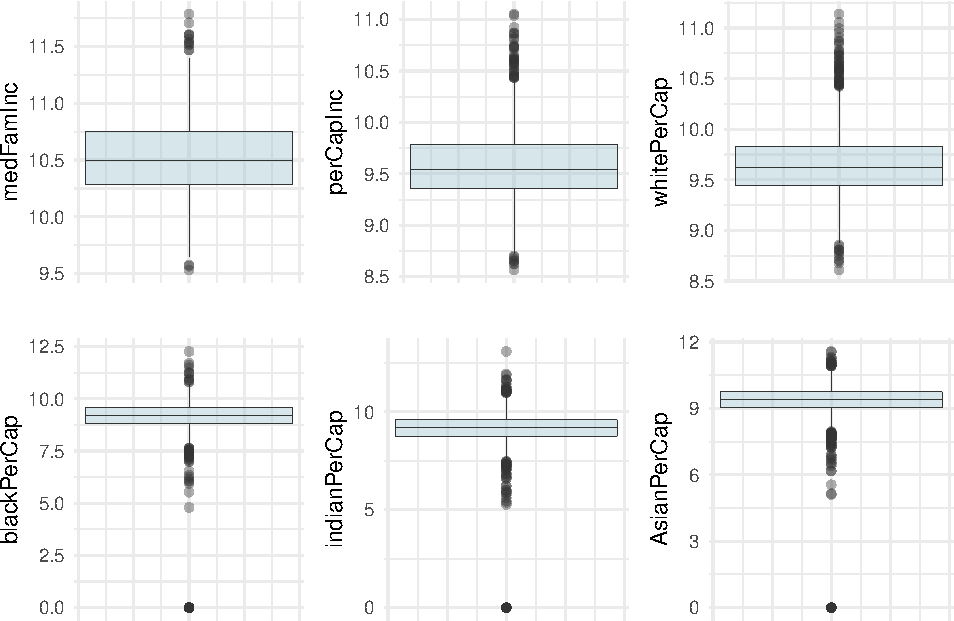
\includegraphics[width=0.75\linewidth]{dissertation_files/figure-latex/Box Plot-1} 

}

\caption{Crime Data: Sample of Boxplots for Visible Outliers}\label{fig:Box Plot}
\end{figure}

The linear correlations among variables have been examined, as shown in
\(Figure XX\). Given the high number of variables, a summary of
correlations is deemed sufficient at this stage. The correlations vary
from negligible to near absolute 1, signifying diverse relationships
among the variables and underscoring the necessity for precise variable
selection.

\begin{figure}[H]

{\centering 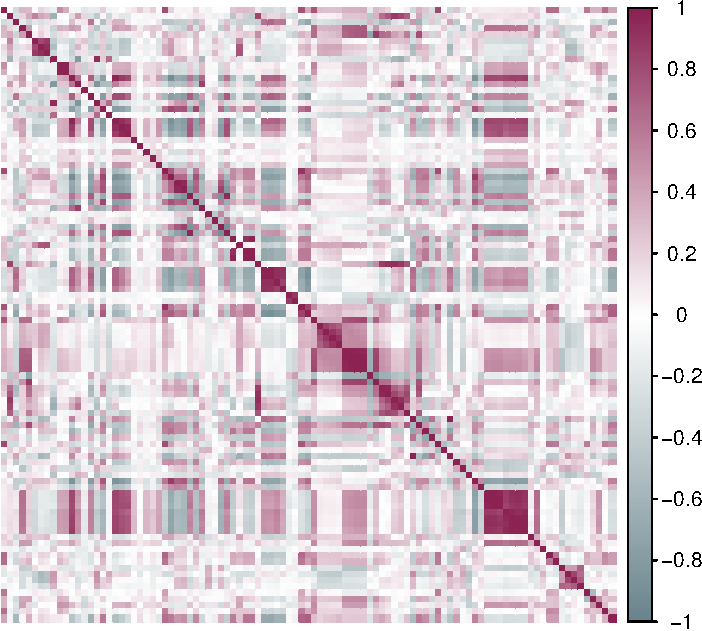
\includegraphics[width=0.70\linewidth]{dissertation_files/figure-latex/Correlations Plot-1} 

}

\caption{Crime Data: Linear Relationship Strength Among Variables}\label{fig:Correlations Plot}
\end{figure}

The scatter plot, see \(Figure XX\), shows a sample of the analysis of
linear correlations between predictors and the target. The correlations
vary, some predictors show a linear relationship with the target.

\begin{figure}[H]

{\centering 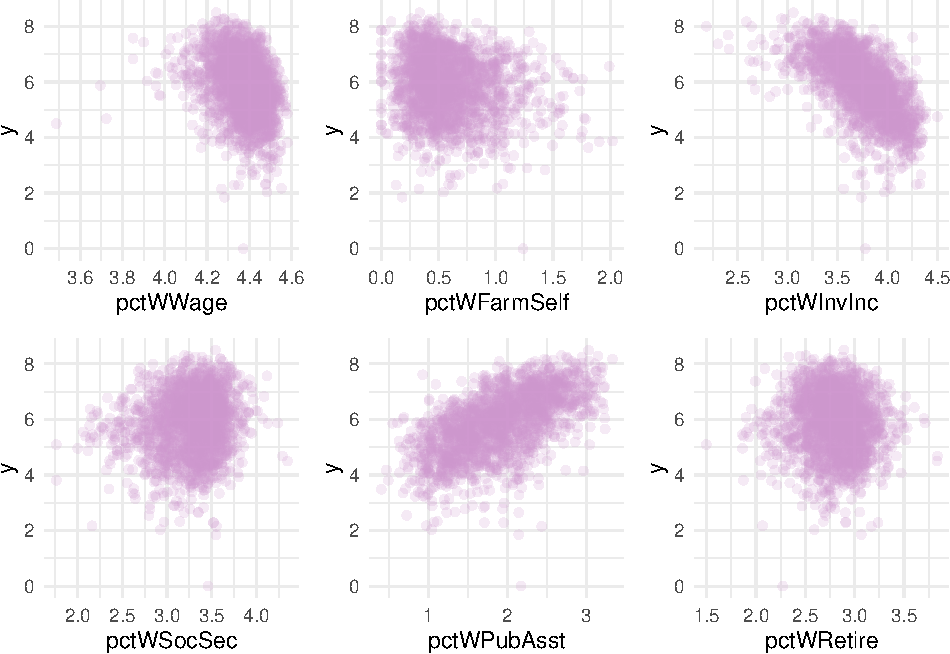
\includegraphics[width=0.75\linewidth]{dissertation_files/figure-latex/Scatter Plot-1} 

}

\caption{Crime Data: Sample Scatter Plot Analysis of Linear Correlations Between Predictors and Target Variable}\label{fig:Scatter Plot}
\end{figure}

With a sizeable sample and apparent relationships between variables and
the target, the next step is applying the methodology that was tested on
simulated data.

In the fitted models, interaction terms are included to examine the
potential joint effects of certain pairs of variables:

The combined influence of the percentage of families with two parents
(PctFam2Par) and the percentage of kids in two-parent households
(PctKids2Par); the percentage of families with two parents (PctFam2Par)
and the total percentage of divorces (TotalPctDiv); vacant boarded
houses (PctVacantBoarded) and the percentage of households without a
phone (PctHousNoPhone) are examined.

Other pairs investigated include the percentage of people in
owner-occupied households (PctPersOwnOccup) with the percentage of
people in densely populated houses (PctPersDenseHous); the percentage of
houses with fewer than three bedrooms (PctHousLess3BR) with median
number of bedrooms per house (MedNumBR); the number of homeless people
in shelters (NumInShelters) and the number of homeless people on the
streets (NumStreet); and the number of vacant houses (HousVacant) with
the percentage of houses that are owner-occupied (PctHousOwnOcc).

Lastly, specific socioeconomic factors are compared with median income,
such as the percentage of families with investment income (pctWInvInc),
the percentage of the population under poverty (PctPopUnderPov),
unemployment rates (PctUnemployed), public assistance rates
(pctWPubAsst), population under poverty (PctPopUnderPov), percentage of
individuals with less than 9th-grade education (PctLess9thGrade), high
school graduation rates (PctNotHSGrad), divorce rates (TotalPctDiv),
families with two parents (PctFam2Par), and the number of kids born to
never married (NumKidsBornNeverMar). Each interaction could provide a
more nuanced understanding of the complex factors influencing crime
rates.

\newpage

\section{Crime Data Study Results}

\newpage

\section{Conclusions}

\newpage

\section{Appendix}

\subsection{Tables}

\begin{longtable}[t]{lll}
\caption{\label{tab:Crime Data Table}Crime Data: Summary of Selected Variables and Their Characteristics for Model Fitting}\\
\toprule
Variable & Included & Type\\
\midrule
\endfirsthead
\caption[]{Crime Data: Summary of Selected Variables and Their Characteristics for Model Fitting \textit{(continued)}}\\
\toprule
Variable & Included & Type\\
\midrule
\endhead

\endfoot
\bottomrule
\endlastfoot
US state & No & Nominal\\
numeric code for county & No & Categorical\\
numeric code for community & No & Categorical\\
community name & No & Text\\
fold number & No & Categorical\\
\addlinespace
population of community & Yes & Continuous\\
mean people per household & Yes & Continuous\\
percentage of population that is african american & No & Continuous\\
percentage of population that is caucasian & Yes & Continuous\\
percentage of population that is of asian heritage & Yes & Continuous\\
\addlinespace
percentage of population that is of hispanic heritage & Yes & Continuous\\
percentage of population that is 12-21 in age & Yes & Continuous\\
percentage of population that is 12-29 in age & Yes & Continuous\\
percentage of population that is 16-24 in age & Yes & Continuous\\
percentage of population that is 65 and over in age & Yes & Continuous\\
\addlinespace
number of people living in areas classified as urban & Yes & Continuous\\
percentage of people living in areas classified as urban & Yes & Continuous\\
median household income & Yes & Continuous\\
percentage of households with wage or salary income in 1989 & Yes & Continuous\\
percentage of households with farm or self employment income in 1989 & Yes & Continuous\\
\addlinespace
percentage of households with investment / rent income in 1989 & Yes & Continuous\\
percentage of households with social security income in 1989 & Yes & Continuous\\
percentage of households with public assistance income in 1989 & Yes & Continuous\\
percentage of households with retirement income in 1989 & Yes & Continuous\\
median family income & Yes & Continuous\\
\addlinespace
per capita income & Yes & Continuous\\
per capita income for caucasians & Yes & Continuous\\
per capita income for african americans & Yes & Continuous\\
per capita income for native americans & Yes & Continuous\\
per capita income for people with asian heritage & Yes & Continuous\\
\addlinespace
per capita income for people with other heritage & Yes & Continuous\\
per capita income for people with hispanic heritage & Yes & Continuous\\
number of people under the poverty level & Yes & Continuous\\
percentage of people under the poverty level & Yes & Continuous\\
percentage of people 25 and over with less than a 9th grade education & Yes & Continuous\\
\addlinespace
percentage of people 25 and over that are not high school graduates & Yes & Continuous\\
percentage of people 25 and over with a bachelors degree or higher education & Yes & Continuous\\
percentage of people 16 and over, in the labor force, and unemployed & Yes & Continuous\\
percentage of people 16 and over who are employed & Yes & Continuous\\
percentage of people 16 and over who are employed in manufacturing & Yes & Continuous\\
\addlinespace
percentage of people 16 and over who are employed in professional services & Yes & Continuous\\
percentage of people 16 and over who are employed in management & Yes & Continuous\\
percentage of people 16 and over who are employed in professional occup. & Yes & Continuous\\
percentage of males who are divorced & Yes & Continuous\\
percentage of males who have never married & Yes & Continuous\\
\addlinespace
percentage of females who are divorced & Yes & Continuous\\
percentage of population who are divorced & Yes & Continuous\\
mean number of people per family & Yes & Continuous\\
percentage of families (with kids) that are headed by two parents & Yes & Continuous\\
percentage of kids in family housing with two parents & Yes & Continuous\\
\addlinespace
percent of kids 4 and under in two parent households & Yes & Continuous\\
percent of kids age 12-17 in two parent households & Yes & Continuous\\
percentage of moms of kids 6 and under in labor force & Yes & Continuous\\
percentage of moms of kids under 18 in labor force & Yes & Continuous\\
number of kids born to never married & Yes & Continuous\\
\addlinespace
percentage of kids born to never married & Yes & Continuous\\
total number of people known to be foreign born & Yes & Continuous\\
percentage of immigrants who immigated within last 3 years & Yes & Continuous\\
percentage of immigrants who immigated within last 5 years & Yes & Continuous\\
percentage of immigrants who immigated within last 8 years & Yes & Continuous\\
\addlinespace
percentage of immigrants who immigated within last 10 years & Yes & Continuous\\
percent of population who have immigrated within the last 3 years & Yes & Continuous\\
percent of population who have immigrated within the last 5 years & Yes & Continuous\\
percent of population who have immigrated within the last 8 years & Yes & Continuous\\
percent of population who have immigrated within the last 10 years & Yes & Continuous\\
\addlinespace
percent of people who speak only English & Yes & Continuous\\
percent of people who do not speak English well & Yes & Continuous\\
percent of family households that are large (6 or more) & Yes & Continuous\\
percent of all occupied households that are large (6 or more people) & Yes & Continuous\\
mean persons per household (numeric - decimal) & Yes & Continuous\\
\addlinespace
mean persons per owner occupied household & Yes & Continuous\\
mean persons per rental household (numeric - decimal) & Yes & Continuous\\
percent of people in owner occupied households (numeric - decimal) & Yes & Continuous\\
percent of persons in dense housing (more than 1 person per room) & Yes & Continuous\\
percent of housing units with less than 3 bedrooms & Yes & Continuous\\
\addlinespace
median number of bedrooms & Yes & Continuous\\
number of vacant households & Yes & Continuous\\
percent of housing occupied & Yes & Continuous\\
percent of households owner occupied & Yes & Continuous\\
percent of vacant housing that is boarded up & Yes & Continuous\\
\addlinespace
percent of vacant housing that has been vacant more than 6 months & Yes & Continuous\\
median year housing units built & Yes & Continuous\\
percent of occupied housing units without phone (in 1990, this was rare!) & Yes & Continuous\\
percent of housing without complete plumbing facilities & Yes & Continuous\\
owner occupied housing - lower quartile value & Yes & Continuous\\
\addlinespace
owner occupied housing - median value & Yes & Continuous\\
owner occupied housing - upper quartile value & Yes & Continuous\\
rental housing - lower quartile rent & Yes & Continuous\\
rental housing - median rent (Census variable H32B from file STF1A) & Yes & Continuous\\
rental housing - upper quartile rent & Yes & Continuous\\
\addlinespace
median gross rent (Census H43A from STF3A - with utilities) & Yes & Continuous\\
median gross rent as a percentage of household income & Yes & Continuous\\
median owners cost as a pct of household income (mortgage) & Yes & Continuous\\
median owners cost as a pct of household income (without mortgage) & Yes & Continuous\\
number of people in homeless shelters & Yes & Continuous\\
\addlinespace
number of homeless people counted in the street & Yes & Continuous\\
percent of people foreign born & No & Continuous\\
percent of people born in the same state as currently living & Yes & Continuous\\
percent of people living in the same house as in 1985 (5 years before) & Yes & Continuous\\
percent of people living in the same city as in 1985 (5 years before) & Yes & Continuous\\
\addlinespace
percent of people living in the same state as in 1985 (5 years before) & Yes & Continuous\\
number of sworn full time police officers & No & Continuous\\
sworn full time police officers per 100K population & No & Continuous\\
number of sworn full time police officers in field operations & No & Continuous\\
sworn full time police officers in field operations & No & Continuous\\
\addlinespace
total requests for police & No & Continuous\\
total requests for police per 100K popuation & No & Continuous\\
total requests for police per police officer & No & Continuous\\
police officers per 100K population & No & Continuous\\
a measure of the racial match between the community and the police force & No & Continuous\\
\addlinespace
percent of police that are caucasian & No & Continuous\\
percent of police that are african american & No & Continuous\\
percent of police that are hispanic & No & Continuous\\
percent of police that are asian & No & Continuous\\
percent of police that are minority of any kind & No & Continuous\\
\addlinespace
number of officers assigned to special drug units & No & Continuous\\
number of different kinds of drugs seized & No & Continuous\\
police average overtime worked & No & Continuous\\
land area in square miles & Yes & Continuous\\
population density in persons per square mile & Yes & Continuous\\
\addlinespace
percent of people using public transit for commuting & Yes & Continuous\\
number of police cars & No & Continuous\\
police operating budget & No & Continuous\\
percent of sworn full time police officers on patrol & No & Continuous\\
gang unit deployed & No & Categorical\\
\addlinespace
percent of officers assigned to drug units & Yes & Continuous\\
police operating budget per population & No & Continuous\\
total number of violent crimes per 100K popuation & Target & Continuous\\*
\end{longtable}

\subsection{Plots}

\textbf{Simulated Data}

\textbf{Crime Data}

\begin{figure}[H]

{\centering 
\includegraphics[width=0.85\linewidth]{dissertation_files/figure-latex/Histograms FULL df Plot-1} 

}

\caption{Crime Data: Histograms Illustrating Variable Distribution Prior to Transformation}\label{fig:Histograms FULL df Plot}
\end{figure}

\subsection{Code}

For the full code, which includes the entire project, please access the
publicly available GitHub repository. The files included are as listed:

\begin{enumerate}
\def\labelenumi{\arabic{enumi}.}
\tightlist
\item
  data\_crime\_raw.R - handling of the Crime data
\item
  simulate\_data.R - Type 1 through Type 4 data simulation
\item
  functions.R - functions for fitting the all methodology
\item
  main.R - main working file
\item
  read.me - text file describing the files contained in the repository
\item
  crime\_raw.csv - copy of the file containing the Crime data
\item
  dissertation.rmd - the dissertation RMarkdown file
\end{enumerate}

\textbf{Snippets of code follow:}

\textbf{Data Simulation}

\textbf{Crime Data}

\textbf{Functions}

\textbf{Main Working File}

\section{List of Figures and Tables}

\listoffigures
  \listoftables

\section{Bibliography}

\hypertarget{refs}{}
\begin{CSLReferences}{1}{0}
\leavevmode\vadjust pre{\hypertarget{ref-Barker2013}{}}%
Barker, R. J., \& Link, W. A. (2013). Bayesian multimodel inference by
RJMCMC: A gibbs sampling approach. \emph{The American Statistician},
\emph{67}(3), 150--156.
\url{https://doi.org/10.1080/00031305.2013.791644}

\leavevmode\vadjust pre{\hypertarget{ref-Bhattacharya2016}{}}%
Bhattacharya, A., Chakraborty, A., \& Mallick, B. K. (2016). \emph{Fast
sampling with gaussian scale-mixture priors in high-dimensional
regression}. \url{http://arxiv.org/abs/1506.04778}

\leavevmode\vadjust pre{\hypertarget{ref-Carlin1995}{}}%
Bradley, P. C., \& Chib, S. (1995). Bayesian model choice via markov
chain monte carlo methods. \emph{Journal of the Royal Statistical
Society: Series B (Methodological)}, \emph{57}, 473--484.
\url{https://doi.org/10.1111/j.2517-6161.1995.tb02042.x}

\leavevmode\vadjust pre{\hypertarget{ref-Carvalho2010}{}}%
Carvalho, C. M., Polson, N. G., \& Scott, J. G. (2010). The horseshoe
estimator for sparse signals. \emph{Biometrika}, \emph{97}, 465--480.
\url{https://doi.org/10.1093/biomet/asq017}

\leavevmode\vadjust pre{\hypertarget{ref-Chen2016}{}}%
Chen, T., \& Guestrin, C. (2016). \emph{XGBoost: A scalable tree
boosting system}. \url{https://doi.org/10.1145/2939672.2939785}

\leavevmode\vadjust pre{\hypertarget{ref-Fan2008}{}}%
Fan, J., \& Lv, J. (2008). Sure independence screening for ultrahigh
dimensional feature space. \emph{Journal of the Royal Statistical
Society. Series B: Statistical Methodology}, \emph{70}, 849--911.
\url{https://doi.org/10.1111/j.1467-9868.2008.00674.x}

\leavevmode\vadjust pre{\hypertarget{ref-Gelling2019}{}}%
Gelling, N., Schofield, M. R., \& Barker, R. J. (2019). R package
rjmcmc: Reversible mump MCMC using post-processing. \emph{Australian and
New Zealand Journal of Statistics}, \emph{61}, 189--212.
\url{https://doi.org/10.1111/ANZS.12263}

\leavevmode\vadjust pre{\hypertarget{ref-Gelman2020}{}}%
Gelman, A., Carlin, J. B., Stern, H. S., Dunson, D. B., Vehtari, A., \&
Rubin, D. B. (2020). \emph{Bayesian data analysis. Third edition} (pp.
165--175).

\leavevmode\vadjust pre{\hypertarget{ref-Green1995}{}}%
Green, P. J. (1995). Reversible jump markov chain monte carlo
computation and bayesian model determination. \emph{Biometrika},
\emph{82}, 711--732. \url{https://doi.org/10.2307/2337340}

\leavevmode\vadjust pre{\hypertarget{ref-Guo2020}{}}%
Guo, R., Zhao, Z., Wang, T., Liu, G., Zhao, J., \& Gao, D. (2020).
Degradation state recognition of piston pump based on ICEEMDAN and
XGBoost. \emph{Applied Sciences}, \emph{10}, 6593.
\url{https://doi.org/10.3390/app10186593}

\leavevmode\vadjust pre{\hypertarget{ref-Hans2007}{}}%
Hans, C., Dobra, A., \& West, M. (2007). Shotgun stochastic search for
"large p" regression. \emph{Journal of the American Statistical
Association}, \emph{102}, 507--516.
\url{https://doi.org/10.1198/016214507000000121}

\leavevmode\vadjust pre{\hypertarget{ref-Hastie2017}{}}%
Hastie, T., Tibshirani, R., \& Friedman, J. H. (2017). \emph{The
elements of statistical learning: Data mining, inference, and
prediction} (2nd Edition). Springer.
\url{http://www.springer.com/series/692}

\leavevmode\vadjust pre{\hypertarget{ref-Hoeting1999}{}}%
Hoeting, J. A., Madigan, D., Raftery, A. E., \& Volinsky, C. T. (1999).
Bayesian model averaging: A tutorial. \emph{Statistical Science},
\emph{14}(4), 382--401. \url{http://www.jstor.org/stable/2676803}

\leavevmode\vadjust pre{\hypertarget{ref-Ishwaran2010}{}}%
Ishwaran, H., Kogalur, U. B., \& Rao, J. S. (2010). Spikeslab:
Prediction and variable selection using spike and slab regression.
\emph{R Journal}, \emph{2}, 68--73.
\url{https://doi.org/10.32614/rj-2010-018}

\leavevmode\vadjust pre{\hypertarget{ref-Ishwaran2005}{}}%
Ishwaran, H., \& Rao, J. S. (2005). Spike and slab variable selection:
Frequentist and bayesian strategies. In \emph{Annals of Statistics}
(Vol. 33, pp. 730--773).
\url{https://doi.org/10.1214/009053604000001147}

\leavevmode\vadjust pre{\hypertarget{ref-jeffreys1935}{}}%
Jeffreys, H. (1935). Some tests of significance, treated by the theory
of probability. \emph{Mathematical Proceedings of the Cambridge
Philosophical Society}, \emph{31}(2), 203--222.
\url{https://doi.org/10.1017/S030500410001330X}

\leavevmode\vadjust pre{\hypertarget{ref-Jianqing2010}{}}%
Jianqing, F., Moore, F. L., \& Jinchi, L. (2010). A selective overview
of variable selection in high dimensional feature space. In
\emph{Statistica Sinica}.

\leavevmode\vadjust pre{\hypertarget{ref-Johnstone2004}{}}%
Johnstone, I. M., \& Silverman, B. W. (2004). Needles and straw in
haystacks: Empirical BAYES estimates of possibly sparse sequences.
\emph{Annals of Statistics}, \emph{32}, 1594--1649.
\url{https://doi.org/10.1214/009053604000000030}

\leavevmode\vadjust pre{\hypertarget{ref-Kahneman2011}{}}%
Kahneman, D. (2011). \emph{Thinking, fast and slow}. Farrar, Straus;
Giroux.

\leavevmode\vadjust pre{\hypertarget{ref-Kannan2015}{}}%
Kaliyaperumal, S. K., Kuppusamy, M., \& Arumugam, S. (2015). Labeling
methods for identifying outliers. In \emph{International Journal of
Statistics and Systems} (Vol. 10, pp. 231--238).
\url{http://www.ripublication.com}

\leavevmode\vadjust pre{\hypertarget{ref-Kass1995}{}}%
Kass, R. E., \& Raftery, A. E. (1995). Bayes factors. \emph{Journal of
the American Statistical Association}, \emph{90}, 773.
\url{https://doi.org/10.2307/2291091}

\leavevmode\vadjust pre{\hypertarget{ref-Vecchi1983}{}}%
Kirkpatrick, S., Gelatt, C. D., \& Vecchi, M. P. (1983). Optimization by
simulated annealing. \emph{Science}, \emph{220}(4598), 671--680.
\url{https://doi.org/10.1126/science.220.4598.671}

\leavevmode\vadjust pre{\hypertarget{ref-Komiyama2018}{}}%
Komiyama, J., Takeda, A., Honda, J., \& Shimao, H. (2018). Nonconvex
optimization for regression with fairness constraints. In J. Dy \& A.
Krause (Eds.), \emph{Proceedings of the 35th international conference on
machine learning} (Vol. 80, pp. 2737--2746). PMLR.
\url{https://proceedings.mlr.press/v80/komiyama18a.html}

\leavevmode\vadjust pre{\hypertarget{ref-Krantz1999}{}}%
Krantz, D. H. (1999). The null hypothesis testing controversy in
psychology. In \emph{Source: Journal of the American Statistical
Association} (Vol. 94, pp. 1372--1381).

\leavevmode\vadjust pre{\hypertarget{ref-Lempers1971}{}}%
Lempers, F. B. (1971). \emph{Posterior probabilities of alternative
linear models: Some theoretical considerations and empirical
experiments}. Rotterdam University Press.

\leavevmode\vadjust pre{\hypertarget{ref-Li2020}{}}%
Li, J. (2020). \emph{When to not use XGBoost?}
\url{https://www.kaggle.com/discussions/general/196542}

\leavevmode\vadjust pre{\hypertarget{ref-Makalic2016}{}}%
Makalic, E., \& Schmidt, D. F. (2016). \emph{High-dimensional bayesian
regularised regression with the BayesReg package}.

\leavevmode\vadjust pre{\hypertarget{ref-Mitchell1988}{}}%
Mitchell, T. J., \& Beauchamp, J. J. (1988). Bayesian variable selection
in linear regression. \emph{Journal of the American Statistical
Association}, \emph{83}, 1023. \url{https://doi.org/10.2307/2290129}

\leavevmode\vadjust pre{\hypertarget{ref-Moran2019}{}}%
Moran, G. E., Ročková, V., \& George, E. I. (2019). Variance prior forms
for high-dimensional bayesian variable selection. \emph{Bayesian
Analysis}, \emph{14}. \url{https://doi.org/10.1214/19-BA1149}

\leavevmode\vadjust pre{\hypertarget{ref-Polson2010}{}}%
Polson, N. G., \& Scott, J. G. (2010). Shrink globally, act locally:
Sparse bayesian regularization and prediction*. In \emph{Bayesian
Statistics 9} (pp. 501--538). Oxford University Press.
\url{https://doi.org/10.1093/acprof:oso/9780199694587.003.0017}

\leavevmode\vadjust pre{\hypertarget{ref-misc_communities_and_crime_unnormalized_211}{}}%
Redmond, M. (2011). \emph{{Communities and Crime Unnormalized}}. UCI
Machine Learning Repository.

\leavevmode\vadjust pre{\hypertarget{ref-Rockova2018}{}}%
Ročková, V., \& George, E. I. (2018). The spike-and-slab LASSO.
\emph{Journal of the American Statistical Association}, \emph{113},
431--444. \url{https://doi.org/10.1080/01621459.2016.1260469}

\leavevmode\vadjust pre{\hypertarget{ref-Rue2001}{}}%
Rue, H. (2001). Fast sampling of gaussian markov random fields.
\emph{Journal of the Royal Statistical Society Series B: Statistical
Methodology}, \emph{63}, 325--338.
\url{https://doi.org/10.1111/1467-9868.00288}

\leavevmode\vadjust pre{\hypertarget{ref-Scutari2022}{}}%
Scutari, M., Panero, F., \& Proissl, M. (2022). Achieving fairness with
a simple ridge penalty. \emph{Statistics and Computing}, \emph{32}, 77.
\url{https://doi.org/10.1007/s11222-022-10143-w}

\leavevmode\vadjust pre{\hypertarget{ref-Shin2015}{}}%
Shin, M., Bhattacharya, A., \& Johnson, V. E. (2015). \emph{Scalable
bayesian variable selection using nonlocal prior densities in
ultrahigh-dimensional settings}. \url{http://arxiv.org/abs/1507.07106}

\leavevmode\vadjust pre{\hypertarget{ref-Spiegelhalter2014}{}}%
Spiegelhalter, D. J., Best, N. G., Carlin, B. P., \& Linde, A. van der.
(2014). The deviance information criterion: 12 years on. In
\emph{Journal of the Royal Statistical Society. Series B (Statistical
Methodology): Vols. 76. No. 3} (pp. 485--493).

\leavevmode\vadjust pre{\hypertarget{ref-Ewout2019}{}}%
Steyerberg, E. W. (2019). \emph{Clinical prediction models: Statistics
for biology and health clinical prediction models a practical approach
to development, validation, and updating second edition}. Springer Cham.
\url{https://doi.org/10.1007/978-3-030-16399-0}

\leavevmode\vadjust pre{\hypertarget{ref-Tadesse2022}{}}%
Tadesse, M. G., \& Vannucci, M. (2022). \emph{Handbook of bayesian
variable selection}. Chapman \& Hall.
\url{https://doi.org/10.1080/00031305.2013.791644}

\leavevmode\vadjust pre{\hypertarget{ref-Tanha2017}{}}%
Tanha, K., Mohammadi, N., \& Janani, L. (2017). P-value: What is and
what is not. \emph{Medical Journal of the Islamic Republic of Iran},
\emph{31}, 377--378. \url{https://doi.org/10.14196/mjiri.31.65}

\leavevmode\vadjust pre{\hypertarget{ref-Tibshirani1996}{}}%
Tibshirani, R. (1996). Regression shrinkage and selection via the lasso.
\emph{Journal of the Royal Statistical Society. Series B
(Methodological)}, \emph{58}(1), 267--288.
\url{http://www.jstor.org/stable/2346178}

\leavevmode\vadjust pre{\hypertarget{ref-Train2012}{}}%
Train, K. E. (2012). \emph{Discrete choice methods with simulation} (2nd
Edition, pp. 284--314). Cambridge University Press.
\url{https://doi.org/10.1017/CBO9780511805271}

\leavevmode\vadjust pre{\hypertarget{ref-Wang2019}{}}%
Wang, J., Xu, J., Zhao, C., Peng, Y., \& Wang, H. (2019). An ensemble
feature selection method for high-dimensional data based on sort
aggregation. \emph{Systems Science and Control Engineering}, \emph{7},
32--39. \url{https://doi.org/10.1080/21642583.2019.1620658}

\leavevmode\vadjust pre{\hypertarget{ref-Zafar2017}{}}%
Zafar, M. B., Valera, I., Rodriguez, M. G., \& Gummadi, K. P. (2017).
Fairness beyond disparate treatment \& disparate impact: Learning
classification without disparate mistreatment. \emph{26th International
World Wide Web Conference, WWW 2017}, 1171--1180.
\url{https://doi.org/10.1145/3038912.3052660}

\leavevmode\vadjust pre{\hypertarget{ref-Zliobaite2011}{}}%
Žliobaitė, I., Kamiran, F., \& Calders, T. (2011). Handling conditional
discrimination. \emph{Proceedings - IEEE International Conference on
Data Mining, ICDM}, 992--1001.
\url{https://doi.org/10.1109/ICDM.2011.72}

\end{CSLReferences}

\end{document}
